\documentclass[11pt]{article}
\usepackage[letterpaper,margin=1in]{geometry}
\usepackage{fontspec}
\usepackage{amsmath,amssymb,amsthm}
\usepackage{graphicx}
\usepackage{booktabs}
\usepackage{multirow}
\usepackage{xcolor}
\usepackage[numbers,sort&compress]{natbib}
\usepackage{microtype}
\usepackage{caption}
\usepackage{subcaption}
\usepackage{enumitem}
\usepackage[hidelinks,pdfusetitle]{hyperref}
\usepackage[section]{placeins}
\captionsetup{font=small,labelfont=bf}
% let tall full-width figures sit near their text instead of drifting to the end
\renewcommand{\topfraction}{0.92}
\renewcommand{\bottomfraction}{0.8}
\renewcommand{\textfraction}{0.07}
\renewcommand{\floatpagefraction}{0.75}
\setcounter{topnumber}{3}
\setcounter{bottomnumber}{2}
\setcounter{totalnumber}{5}
\setlist{itemsep=2pt,topsep=4pt}
\newtheorem{proposition}{Proposition}
\newcommand{\R}{\mathbb{R}}
\newcommand{\ShuffleSnap}{ShuffleSnap}
\newcommand{\RealBalancedExcess}{0.002\%}

\hypersetup{pdftitle={ShuffleSnap: strided windowed exact reassignment for point-to-grid layout, evaluated against certified optima},
            pdfauthor={Draft}, pdfsubject={Point-to-grid assignment},
            pdfkeywords={linear assignment, optimal transport, grid layout, UMAP, visualization}}

\title{\ShuffleSnap: strided windowed exact reassignment for point-to-grid layout,\\ evaluated against certified optima}
\author{Draft --- author list to be decided}
\date{September 2026}

\begin{document}
\maketitle

\begin{abstract}
Snapping each point of a 2D embedding (such as a UMAP layout) to its own cell of a grid,
while minimizing total squared displacement, is a linear assignment problem. Dense solvers
cannot handle it beyond a few tens of thousands of points. We develop and test
\ShuffleSnap, a local search inspired by Shellsort. At a decreasing sequence of strides, it
splits the grid into interleaved subgrids and solves small exact assignment problems in
shifted $8\times8$ windows of each. Every window solve starts from dual potentials derived
in closed form from per-axis optimal transport, which makes it 2--5$\times$ faster than a
standard Hungarian solver with the same results.

To measure true optimality gaps, we built a certified exact solver. It solves min-cost flow
on sparse candidate edges and proves the result optimal for the full, dense problem with a
dual bound evaluated over all cells. Started from \ShuffleSnap, it proved optimality on
every instance we tried, up to $10^6$ points.

On held-out instances with $10^5$ points, \ShuffleSnap\ is within 0.06\% of the optimum on
nine of ten distributions, in a median of 2.3\,s on one core or 0.19\,s on 24 threads.
Its fast and default presets take about as long as BSP-OT with 16 and 64 plans, and at equal
time they are closer to the optimum on eight and nine of the ten distributions. BSP-OT with
64 plans is 3.7--36\% above the optimum on five of them, and RasterFairy is 17--425\% above it
on seven. SciPy's dense exact solver already needs up to 6 minutes at $10^4$ points. On one
workstation, \ShuffleSnap\ also handled a billion points: using 53\,GiB, it passed a six-hour
run of an earlier implementation after 44 minutes and converged after 1\,h\,43\,min, while a
single-plan BSP-OT ended 8.2\% above it.

The method's limits are structural. Its error consists of long closed loops of one-cell
shifts that no window can remove, and we construct inputs on which its relative gap is
unbounded. Uniform points remain the hardest common input (0.8\% at $10^5$).
Bisection starts make results worse, and polishing at coarser strides changes almost
nothing. Warm-started from \ShuffleSnap, the certified solver reaches proven optima in
seconds to minutes at $10^5$ points.

On two real UMAP embeddings, \ShuffleSnap\ is within 0.002\% of the optimal displacement.
There, displacement and neighbourhood preservation diverge: BSP-OT is 2--7\% above the
optimal displacement but halves the fraction of preserved grid neighbours. We release the
implementation, all experiment code and the raw results.
\end{abstract}

\section{Introduction}
\label{sec:intro}

A common way to show a large image or document collection is to embed the items in
the plane (for example with t-SNE~\citep{vandermaaten2008tsne} or
UMAP~\citep{mcinnes2018umap}) and then snap every item to its own cell of a regular grid,
so that thumbnails tile the screen without overlap. Snapping is an assignment problem:
each point must receive a distinct cell, and we would like points to move as little as
possible. Measured as total squared displacement, the best snapping is a linear
assignment problem (LAP), and also a discrete optimal-transport problem with quadratic
cost~\citep{peyre2019computational}.

For a few thousand points, practitioners solve this LAP exactly with a dense
Jonker--Volgenant or Hungarian solver~\citep{markovtsev2017jvtsne,mcdonald2016cloudtogrid,
markovtsev_lapjv,kazmar_lap}. The dense cost matrix needs $8N^2$ bytes, which is
80\,GB at $N=100{,}000$, so these solvers stop being usable somewhere between
10{,}000 and 30{,}000 points. Beyond that, people turn to recursive-splitting heuristics
such as RasterFairy~\citep{klingemann2015rasterfairy} or to fast approximate transport
such as BSP-OT~\citep{genest2025bspot}.

This paper develops and evaluates \ShuffleSnap, a simple heuristic for this regime,
taking its name from Shellsort~\citep{shell1959highspeed}. Shellsort sorts interleaved
subsequences at a decreasing sequence of gaps. \ShuffleSnap\ does the same in 2D: at stride $s$
it splits the grid into $s^2$ interleaved subgrids and solves small \emph{exact}
assignment problems inside $6\times6$ windows of each subgrid, halving $s$ until it
reaches 1 (Figure~\ref{fig:method}). All work is at full resolution; nothing is
aggregated or downsampled.

We treat the idea as a hypothesis to test, not a result to promote. Our aim throughout
was to find where it fails. The main contributions are:

\begin{itemize}
\item \textbf{A careful implementation} of the specified baseline, with documented
  boundary, rectangular-grid, surplus-cell and mask rules. It is a parallel C++ kernel
  with a Python API whose results do not depend on the number of threads.
\item \textbf{A certified exact solver that scales to $10^5$ points.} It solves min-cost
  flow on sparse candidate edges, then prices every edge of the \emph{dense} problem
  through a Lagrangian bound, adding edges until the bound meets the primal cost. It
  gives true optimality gaps, not progress relative to our own best answer, for every
  instance up to 200{,}000 points in this study. In our experiments it is also a strong
  practical baseline.
\item \textbf{Measured improvements and non-improvements.} On a held-out development set,
  a finer stride sequence (ratio $\sqrt2$ instead of 2) and larger windows reduce the
  excess cost severalfold for a small time increase. Several intuitive ideas make things
  \emph{worse}: sorted or bisection starts, polishing at coarser strides, and a
  Jonker--Volgenant window solver.
\item \textbf{A diagnosis of the remaining error.} The gap to the optimum is concentrated
  in a few long closed loops of points, each displaced by about one cell. No window
  smaller than a loop can remove it. Masks with concave bays and grids with surplus
  cells expose the same mechanism at a larger scale.
\item \textbf{A benchmark against exact LAP, RasterFairy and BSP-OT.} We first verified
  each comparator's capabilities: we found and worked around coordinate truncation in the
  PyPI release of RasterFairy, and used its much stronger upstream version. The
  benchmark covers varied and adversarial distributions, masks, prime point counts, two
  real UMAP embeddings with 70{,}000 points each, multiple seeds, matched-budget curves,
  and scaling to $10^6$ points. We report cost, time, peak memory, and neighbourhood
  preservation, and we keep displacement and neighbourhood measures separate.
\end{itemize}

The implementation (\texttt{shufflesnap}) and this paper's experiment code, raw results
and figure scripts are released as two separate repositories.

\section{Problem}
\label{sec:problem}

\paragraph{Cells.} A target is a boolean mask on a $W\times H$ lattice. Lattice position
$(x,y)$ is column $x$ and row $y$, and usable positions are the cells
$c_1,\dots,c_M$. Cell centers default to the integer coordinates, so one unit is one cell
pitch. Anisotropic pitches (e.g.\ for 4:3 thumbnails) scale the centers but leave the
lattice unchanged. A full rectangle, a rectangle whose last row is only partly usable,
a disk, a ring, and the shape of a letter are all masks.

\paragraph{Points and normalization.} Input points $q_1,\dots,q_N$ ($N\le M$) are mapped
into the cell frame before anything else. Unless stated otherwise, each axis of the
point bounding box is mapped affinely onto the bounding box of the usable cell centers
(\emph{bbox} normalization); $p_i$ denotes the mapped points. The mapping is part of the
problem: in every comparison, all methods receive identical $p_i$ and identical cell
centers.

\paragraph{Objective.} We seek an injective assignment $\sigma:\{1..N\}\to\{1..M\}$
minimizing
\begin{equation}
  C(\sigma) = \sum_{i=1}^N \lVert p_i - c_{\sigma(i)}\rVert^2 .
  \label{eq:cost}
\end{equation}
When $N=M$ this is a bijection. When $N<M$ the solver must also decide which $M-N$ cells
stay empty. Unlike the bijective case, the cell term $\sum_i \lVert c_{\sigma(i)}\rVert^2$
then depends on the choice, so the surplus case is not just a relabelling of the
bijective one.

\paragraph{A certificate of optimality.} Equation~\eqref{eq:cost} is the linear program
$\min \sum_{ij} c_{ij}x_{ij}$ with $\sum_j x_{ij}=1$ for every point,
$\sum_i x_{ij}\le1$ for every cell, and $x\ge0$, where $c_{ij}=\lVert p_i-c_j\rVert^2$.
Its constraint matrix is totally unimodular. We use the following elementary bound.

\begin{proposition}\label{prop:lb}
For any cell potentials $v\in\R^M$,
\[
  \mathrm{LB}(v) = \sum_{i=1}^N \min_{j} \bigl(c_{ij}-v_j\bigr) + \sum_{j=1}^M v_j - (M-N)\max_j v_j
\]
is a lower bound on the optimal cost. The bound is tight (equals the optimum) for
optimal dual potentials.
\end{proposition}
\begin{proof}
Let $\bar v=\max_j v_j$ and $v'_j=v_j-\bar v\le0$. Let $u_i=\min_j(c_{ij}-v'_j)$. Then
$(u,v')$ is feasible for the dual $\max\sum_i u_i+\sum_j v'_j$ subject to
$u_i+v'_j\le c_{ij}$ and $v'\le0$, and its objective equals $\mathrm{LB}(v)$ (shifting all
potentials by $\bar v$ changes every $u_i$ by $+\bar v$ and the cell sum by $-M\bar v$).
Weak duality gives the bound. Strong duality of the LP gives tightness.
\end{proof}

The bound needs a minimum over \emph{all} $M$ cells for every point. It does not depend
on how $v$ was obtained, so $C(\sigma)-\mathrm{LB}(v)$ certifies the gap of any
assignment $\sigma$. We use it for every ``excess over optimum'' number in this paper,
and we never measure progress relative to our own final cost.

\paragraph{Reporting error.} We report the \emph{relative excess}
$C(\sigma)/C^\star-1$ and the \emph{absolute excess per point} $(C(\sigma)-C^\star)/N$ in
cell units squared, where $C^\star$ is a certified optimum. Both are needed.
Inputs that already lie almost on the cells have a tiny $C^\star$, which makes
relative numbers explode. Inputs dominated by outliers (heavy tails) have a huge
$C^\star$, which makes every method look perfect in relative terms.

\section{Related work}
\label{sec:related}

\paragraph{Exact assignment.} The Hungarian method~\citep{kuhn1955hungarian,munkres1957algorithms}
and shortest-augmenting-path variants such as Jonker--Volgenant
(JV)~\citep{jonker1987shortest} solve dense $N\times N$ problems in $O(N^3)$ time and
$O(N^2)$ memory. SciPy's \texttt{linear\_sum\_assignment} implements a modified JV
without initialization~\citep{crouse2016implementing,virtanen2020scipy}. The
\texttt{lap} and \texttt{lapjv} packages provide dense JV with heuristic initialization
(\texttt{lap} also provides a sparse variant)~\citep{kazmar_lap,markovtsev_lapjv}.
Auction algorithms~\citep{bertsekas1979distributed,bertsekas1988auction} and cost-scaling
push--relabel~\citep{goldberg1995efficient} handle sparse problems. The min-cost-flow
solver in OR-Tools, which we use, is a cost-scaling push--relabel
method~\citep{ortools,ortools_mincostflow_doc}. \citet{burkard2009assignment} survey the
field. Geometric bipartite matching admits near-linear $\varepsilon$-approximations in
theory~\citep{sharathkumar2012transportation,raghvendra2020nearlinear}. We know of no
practical implementations aimed at this use case.

\paragraph{Optimal transport.} With quadratic cost, optimal maps are gradients of
convex functions~\citep{brenier1991polar}. Least-squares assignments with prescribed
cluster sizes are exactly those induced by power
diagrams~\citep{aurenhammer1998minkowski}, the geometric fact behind semi-discrete
solvers~\citep{merigot2011multiscale,levy2015numerical} and behind the potentials in our
certificate. Multiscale methods solve coarsened problems and refine
them~\citep{merigot2011multiscale,schmitzer2016sparse,gerber2017multiscale}. Schmitzer's
sparse multiscale algorithm in particular alternates sparse subproblems with global
optimality checks~\citep{schmitzer2016sparse}, as our exact solver does. Entropic
regularization~\citep{cuturi2013sinkhorn} and sliced
transport~\citep{rabin2012wasserstein,bonneel2015sliced} trade exactness for speed; see
\citet{peyre2019computational} for a survey. BSP-OT~\citep{genest2025bspot} builds many
randomized binary space partition matchings in $O(N\log N)$ and merges them with a
cycle-based rule. Its official code~\citep{genest2025bspotcode} has Python
bindings~\citep{takayama2026bspotpython,flamary2026potsoftware}. The BSP-OT paper does
not evaluate uniform grid targets.

\paragraph{Grid layouts for visualization.} RasterFairy~\citep{klingemann2015rasterfairy}
recursively slices the point cloud and the target raster in matching proportions, and
supports masks and hexagonal rasters. Its current upstream version also solves small
leaf blocks exactly (Section~\ref{sec:setup}). IsoMatch~\citep{fried2015isomatch}
projects with Isomap and then solves a dense Hungarian problem, which it names as its
bottleneck. Kernelized sorting~\citep{quadrianto2008kernelized,quadrianto2010kernelized},
self-organizing maps~\citep{kohonen1982selforganized}, the Self-Sorting
Map~\citep{strong2014selfsorting}, and Linear Assignment Sorting and its fast variant
FLAS~\citep{barthel2023improved} arrange high-dimensional items directly on a grid.
LAS repeatedly solves full JV problems between features and smoothed map vectors.
Gridfit~\citep{keim1998gridfit} and DGrid~\citep{hilasaca2024grid} remove overlap in
scatterplots by hierarchical partitioning. These methods mostly optimize neighbourhood
preservation, and they measure it with trustworthiness and
continuity~\citep{venna2001neighborhood,venna2006local} or the Distance Preservation
Quality~\citep{barthel2023improved}. We keep that goal distinct from displacement:
the LAP objective only minimizes how far points move.

\paragraph{Sorting networks and Shellsort.} Shellsort~\citep{shell1959highspeed} sorts
with insertion-sort passes over a decreasing sequence of gaps, so early passes move
elements far and late passes move them little. \ShuffleSnap\ borrows this schedule.
Unlike Shellsort's final gap-1 pass, however, its final stride-1 stage is not guaranteed
to reach the optimum. That difference turns out to be the heart of the matter
(Section~\ref{sec:anatomy}).

\section{\ShuffleSnap}
\label{sec:method}

\begin{figure}[tbp]
  \centering
  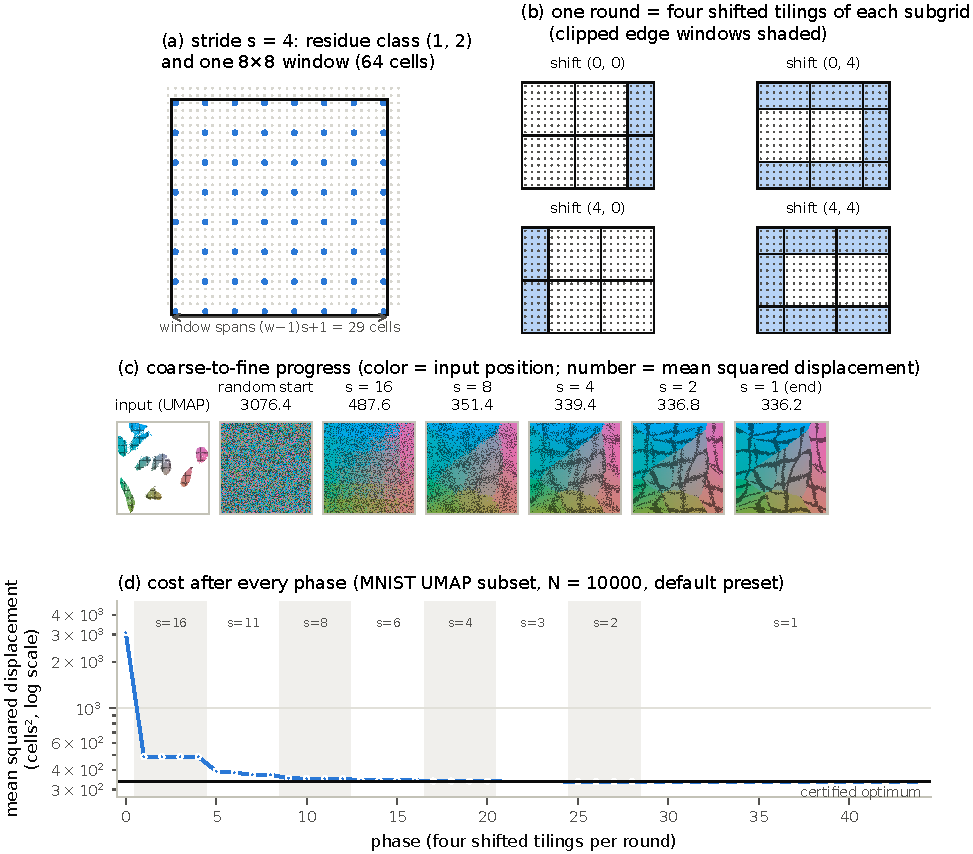
\includegraphics[width=\linewidth]{figures/fig_method.pdf}
  \caption{How \ShuffleSnap\ works. (a)~At stride $s=4$ the lattice splits into
  $s^2=16$ interleaved residue subgrids. Blue marks one of them. An $8\times8$ window of
  that subgrid (filled blue) holds 64 cells spaced 4 apart and spans 29 cells. The
  occupants of those 64 cells are reassigned among the same cells by an exact linear
  assignment. (b)~Each round tiles every subgrid four times, with the tiling shifted by
  half a window in $x$, $y$, or both, so that window borders move. Windows that cross the
  subgrid edge are clipped (shaded), never dropped, on all four sides. (c)~Progress on a
  10{,}000-point subset of a UMAP embedding of MNIST. Each point is colored by its
  \emph{input} position, and the dark bands are the lines of a square grid drawn on the
  input (graph paper). Both travel with the points, so a smooth color field and unbroken
  lines mean the input neighbourhood structure survived; every second stride is shown.
  (d)~Mean squared displacement after every phase. The coarse strides remove most of the
  cost; the stride-1 rounds that follow change little.}
  \label{fig:method}
\end{figure}

\subsection{The algorithm}
\label{sec:algorithm}

\ShuffleSnap\ has two main parameters, the window side $w$ and the stride ratio $r$. The
default is $w=8$ and $r=\sqrt2$ (Section~\ref{sec:improve}).
\begin{enumerate}
\item \textbf{Start.} Place the $N$ points on a uniformly random subset of $N$ cells, as a
  seeded random permutation.
\item \textbf{Strided windows.} At stride $(s_x,s_y)$, lattice positions with the same
  residues $(x \bmod s_x,\, y\bmod s_y)$ form a subgrid, for $s_x s_y$ subgrids in
  total. In its own coordinates each subgrid is tiled with $w\times w$ windows. A window
  therefore contains at most $w^2$ cells (64 by default), spaced $s$ apart on the lattice
  and spanning $(w-1)s+1$ cells per axis.
\item \textbf{Exact reassignment.} In every window, the points currently occupying its
  cells are reassigned among the same cells, empty ones included, by solving the dense
  linear assignment on squared distances to the original (normalized) coordinates. The
  window's cell set never changes, so the global assignment stays injective.
\item \textbf{Shifted tilings.} The tiling is repeated with shifts $(0,0)$, $(0,w/2)$,
  $(w/2,0)$ and $(w/2,w/2)$ in subgrid coordinates. These four phases form one round.
  Windows in one phase are disjoint and are solved in parallel.
\item \textbf{Schedule.} On an axis of length $L$, the first stride is the smallest power of
  two with $ws\ge L$, so that the first windows span the grid. After one round, both strides
  are divided by $r$ and rounded, with repeats removed and never below 1. Stride-1 rounds
  then repeat until a full round moves no point, or until a time budget runs out.
\end{enumerate}
With $r=2$ the strides halve, and every level quarters the area a window spans. With
$r=\sqrt2$ the area halves from one level to the next, so each level starts from a layout
that is already sorted at nearly its own scale; this plausibly explains why $\sqrt2$ works
well (Section~\ref{sec:ablation}). It roughly doubles the number of levels.

\paragraph{Window solver and acceptance.} Each window is a rectangular problem: $k$
occupants and $m\ge k$ cells, with $m\le w^2$. We solve it exactly by
shortest augmenting paths with dual potentials (the Hungarian method, $O(k^2m)$ time),
started from duals built from the window's geometry (Section~\ref{sec:geosolver}). A new window assignment replaces the old
one only if it is cheaper by more than a relative $10^{-12}$. Because the old assignment
is feasible for the window problem, every accepted change strictly lowers the global
cost by at least that margin. Hence the cost sequence is monotone, the search
terminates, and ties (e.g.\ duplicated points) never cause cycling.

\subsection{A geometric window solver}
\label{sec:geosolver}

Almost all of the running time is spent in window solves, so the choice of solver matters. Generic
LAP solvers are slow on these windows for a geometric reason. On clustered data, and at
coarse strides in particular, a window's occupants often come from a dense cluster that
lies far from most of the window's cells. Seen from far away, every point prefers the same
corner cell. The usual greedy start (match each row to its cheapest free column) then
matches little, and the shortest augmenting paths become long. We captured about
79{,}000 windows from runs with $8\times8$ windows and $r=\sqrt2$ (20{,}000 points; unchanged
windows skipped as in the kernel). In 96\% of the MNIST windows with at least 16 points, the
points' cheapest cells numbered at most half as many as the points (median: one cheapest
cell per 3.6 points). On uniform points this happened in 1\% of the windows.

The squared-distance structure offers a better start. For the cost $|p-q|^2$, optimal
duals on the cells are a discretized Brenier potential~\citep{brenier1991polar}: $v(q)=|q|^2-2\psi(q)$ with $\psi$
convex, and $\nabla\psi$ maps cells to the points that occupy them. We use the potential
of a map that is optimal per axis. On one axis, the optimal transport between the points'
and the cells' coordinates is the sorted order, and its potential is piecewise linear:
between consecutive distinct cell coordinates, $\psi$ increases at a rate equal to the
point quantile at that cumulative cell mass. Summing the two axes gives separable starting
duals in $O(k\log k+m\log m)$ time. They move a distant cluster onto the window and
spread it over the window's rows and columns, which removes most of the conflicts. The
solver then proceeds in four exact steps:
\begin{enumerate}
\item row reduction under the starting duals, and a greedy match of every row whose
  cheapest column is still free;
\item a column reduction, which keeps the duals feasible and makes every cell tight for at
  least one point;
\item Kuhn's augmenting paths restricted to tight (zero reduced cost) edges, for the rows
  still unmatched;
\item shortest augmenting paths for the rest (Dijkstra over a shrinking list of unscanned
  columns with lazy dual updates, ties broken towards free columns, as in
  SciPy's solver~\citep{crouse2016implementing}).
\end{enumerate}
Arbitrary starting duals are valid only for a square problem. A window with empty cells is
therefore either padded with zero-cost rows and solved from the geometric start, or, if
fewer than half of its rows compete for a cell under zero duals (as on near-uniform data),
solved directly as a rectangular problem from zero duals. Padding such a window would cost
one augmenting path per empty cell.

On the captured windows, the solver returned the optimum on every window. It was 5.1--5.6$\times$ faster
than the Hungarian method with a greedy start on MNIST and mixture windows, and
1.9$\times$ faster on uniform ones. In full runs with the default $8\times8$ windows it is
5.1--5.3$\times$ faster on clustered inputs and 2.0--2.1$\times$ faster on uniform points, on 1
or 24 threads (Section~\ref{sec:ablation}). Its results are identical to the other exact
solvers' up to ties.
\subsection{Implementation}
\label{sec:impl}

The kernel is C++17, exposed to Python with nanobind, and parallelized with OpenMP over
the windows of a phase. Each thread keeps its own scratch buffers. Because windows in a
phase are disjoint and each solve is deterministic, the result is bit-identical for any
thread count; a test checks this. We also track, for every cell, the last phase that
changed its occupant. A window whose cells are unchanged since it was last solved in the
same stage is already optimal, and skipping it does not change the result (also tested).
This matters in the stride-1 convergence rounds, where most windows are untouched. The
cost is recomputed exactly after every phase, which gives an anytime trace, and a time
budget is checked between windows. A serial reference of about 70 lines of NumPy and SciPy
(Appendix~\ref{app:reference}) returns exactly the kernel's assignments and serves as an
executable specification. There is no just-in-time compilation, so nothing is compiled at run time. Compiling the
extension takes 2.6\,s with parallel Ninja (8.1\,s on one core). A complete isolated wheel
build, including creating the build environment as \texttt{pip install} does from source,
takes about 35\,s.

\paragraph{Work per level.} A phase at stride $s$ has about $M/w^2$ windows (plus clipped
ones), each an $O(w^6)$ Hungarian solve in the worst case. The work per phase is
therefore $O(Mw^4)$, independent of $s$, and a schedule with $\ell$ levels costs
$O(\ell M w^4)$ plus the convergence rounds. With $\ell=O(\log L)$ this is
$O(M\log M)$ for fixed $w$. The constant depends strongly on the data: windows far from
optimal need long augmenting paths.

\subsection{Choosing the parameters}
\label{sec:improve}

We chose every setting on a development set (instance seed 0: 23 instances of 10{,}000 to
100{,}000 points, including masks and surplus cells, five start seeds each) and report
every claim on held-out seeds (Section~\ref{sec:ablation}).

\begin{itemize}
\item \textbf{Window size} is the main quality knob. We tried window sides from 6 to 24
  with four stride ratios (35 configurations). Every step up in window size lowered the
  excess, and the gains did not level off: from $8\times8$ to $12\times12$ to $16\times16$
  windows, each step cost 2--2.6 times the time and removed one half to two thirds of the
  remaining excess. There is no sweet spot, so we place three presets along the curve, two of
  them where they can be compared with BSP-OT at equal time: \emph{fast} ($5\times5$ windows)
  takes about as long as BSP-OT with 16 plans, its default, and \emph{balanced} ($8\times8$,
  our default) about as long as BSP-OT with 64 plans, on one core at $10^5$ points.
  \emph{Quality} ($12\times12$) is one step further. For the fast preset, $5\times5$ windows
  with ratio $\sqrt2$ beat $6\times6$ windows with halving strides, which take the same time,
  on five of seven development instances. Windows up to $32\times32$ can be set explicitly. The cost of a window
  solve grows as $w^6$ in the worst case, but a phase has $M/w^2$ windows and most of them
  are nearly sorted or skipped; in our runs the total time grew as about $w^{1.9}$ (uniform)
  to $w^{2.8}$ (clustered data). Using small windows at coarse strides and large ones at
  stride 1 was worse than using large windows throughout.
\item \textbf{Stride ratio.} Dividing strides by $\sqrt2$ instead of 2 (rounded, duplicates
  removed) roughly doubles the number of levels, each at about the same cost, and was on
  or next to the best time--quality trade-off at every window size. Ratios of 1.68 and
  1.19 were close; 2 and 3 were clearly worse.
\item \textbf{Start.} Structured starts are mostly \emph{worse} than a random
  permutation: bisection (the recursive median split used by RasterFairy-like methods) on
  every input, and row sorting on most. They create straight seams that the local windows
  cannot repair. The random start is a decorrelating device, not a lazy default.
\item \textbf{Solver.} All solvers we tried are exact, so they change only time. JV with
  augmenting row reduction is slower than the Hungarian method on these windows,
  because squared distances create many near-ties. An $\varepsilon$-scaled auction whose
  prices warm-start the same exact shortest-path finish is 2--3$\times$ faster on clustered
  data but not on uniform points. The geometric solver (Section~\ref{sec:geosolver}) is the
  fastest on every input. Variants that did not pay off, measured on the captured
  windows: starting duals from an affine or a full-covariance Gaussian map (both worse than
  the per-axis quantile map), duals integrated from the current assignment (better on
  clustered windows, worse on uniform ones, and choosing per window cost more than it
  saved), an auction refinement of the geometric start, repeated row and column
  reductions, and a branch-free scan of all columns in the shortest-path step.
\item \textbf{Post-processing.} Extra stride-2 and stride-1 rounds after convergence changed
  nothing on seven of nine held-out instances (a stride-2 window cannot move a point by one
  cell).
  Merging independent runs component by component, the rule BSP-OT uses, helps less per
  unit time than a larger window.
\end{itemize}

\section{A certified exact solver for large instances}
\label{sec:exact}

Excess over the optimum is only meaningful with a trustworthy optimum. At
$N=100{,}000$ a dense matrix does not fit in memory. SciPy's sparse LAPJV on a
16-nearest-cell graph did not finish a 10{,}000-point instance in eight minutes; we
later found that such graphs are usually \emph{infeasible}, because some cells are not
among any point's 16 nearest. We therefore built a solver that never forms the dense
problem, yet certifies optimality against it.

\begin{enumerate}
\item \textbf{Candidates.} Give each point its 12 nearest cells, plus the $5\times5$
  lattice neighbourhood of its cell in a starting assignment. Including the starting
  assignment guarantees that a perfect matching exists.
\item \textbf{Sparse solve.} Solve the min-cost flow (points $\to$ cells $\to$ sink,
  unit capacities) with OR-Tools' cost-scaling solver. The solver needs integer costs,
  so we scale by $S=2^{56}/((N{+}M{+}2)\max c)$ and round.
  (We found by probing that a scale of $2^{58}/((N{+}M)\max c)$ is accepted and
  $2^{60}/((N{+}M)\max c)$ is rejected with \texttt{BAD\_COST\_RANGE}.)
\item \textbf{Potentials.} For the sparse optimum $\sigma$, build a graph on cells with
  an arc $\sigma(i)\to j$ of weight $c_{ij}-c_{i\sigma(i)}$ for every candidate edge.
  Shortest-path distances from a virtual source joined to all cells give potentials
  $v$ that satisfy complementary slackness on every candidate edge, with $v=0$ on empty
  cells. We compute them in exact integer arithmetic with a label-correcting algorithm.
\item \textbf{Global pricing.} Evaluate $\mathrm{LB}(v)$ (Proposition~\ref{prop:lb}) over
  \emph{all} cells. Cells are grouped into $16\times16$ blocks, and a block is scanned
  only if $\mathrm{dist}^2(p_i,\text{block})-\max_{\text{block}}v$ could beat the best
  value found so far. The pass also lists every cell whose reduced cost undercuts the
  point's current cell. If the bound meets the cost, stop. Otherwise add those edges,
  plus the $3\times3$ neighbourhood of each such point's best-priced cell, and go back
  to step 2.
\end{enumerate}

The certificate is the gap $C(\sigma)-\mathrm{LB}(v)$, computed in floating point from
real-valued costs. It is valid whatever errors occur in steps 1--3. Integer rounding
can only loosen it, by at most $4N/S$ in total; we count an instance as certified when
the gap is at most $\max(10^{-9}C, 4N/S)$. The result is therefore the exact optimum of
the dense problem, whatever candidate edges it started from; the start affects only the
time. Wherever SciPy's dense solver fits, both found the same optimum: on 600 small
instances ($N\le2{,}500$, five distributions, three grid types) to relative $10^{-9}$
(Section~\ref{sec:correctness}), and on all ten distributions at $N=10^4$ to relative
$10^{-10}$.

\paragraph{A pitfall.} Our first version flagged a ``negative cycle'' on some clustered
instances with masks. It declared a cycle once a node had been queued more than $n$
times, which is only valid for FIFO Bellman--Ford, not with the small-label-first queue
we use. The fix is to verify a suspected cycle by walking parent pointers. A regression
test covers it.

\paragraph{Cost.} Started from \ShuffleSnap, the solver reached a certificate on every
instance we gave it: the 232 reference instances (up to 200{,}000 points), every timed run,
and uniform instances up to $10^6$ points. Started from bisection, it failed on 4 of 10
instances at $10^5$ points (Section~\ref{sec:main}). The number of pricing rounds was 1 for
uniform inputs, up to about 8 for clustered, curved or masked inputs, and up to 13 for the
input with 16 heavily duplicated sites. Massive ties are the slowest case: one
such 100{,}000-point instance took 34 minutes, while the median 100{,}000-point
reference took under 3 minutes (six references were computed in parallel).
Section~\ref{sec:results} reports its running time and memory next to the heuristics.
The solver needs a feasible starting assignment. We use \ShuffleSnap's default preset,
and at $10^5$ points we also run it from a bisection start, to separate the two methods'
contributions.

\section{Experimental setup}
\label{sec:setup}

\paragraph{Hardware and software.} All runs used one workstation: an Intel Core
i9-12900KS (8 performance and 8 efficiency cores, 24 hardware threads), 62\,GB RAM,
Ubuntu 24.04 (Linux 6.8), Python 3.12.3, NumPy 2.5.3, SciPy 1.18.1, OR-Tools 9.15,
GCC 13.3 with \texttt{-O3} and no \texttt{-march=native} (portable build). The GPU was
not used. Exact versions and commit hashes are stored with every raw result.
\emph{Single-thread} runs were pinned to one performance core (\texttt{taskset -c 8}) with
all thread pools set to 1. \emph{Multi-thread} runs used all 24 hardware threads without
pinning. For \ShuffleSnap\ this was faster on this machine than using only the 16
performance-core threads (Section~\ref{sec:threads}). The machine also ran unrelated background services
(load average about 1). Benchmarks ran sequentially, only after all reference optima had
been computed.

\paragraph{Timing and memory boundaries.} Every run is a fresh process. The timer
brackets exactly one call of the method adapter. It includes all method-specific work:
cost matrices, trees, starts, the method's own normalization, and format conversion. It
excludes instance generation, the common normalization, validation, and metrics. Before
the timed call, each method is run once on a 256-point instance. This takes imports,
lazy initialization and thread-pool start-up out of the timing; that warm-up time is
recorded separately and is below 0.3\,s for every method. None of the methods uses
just-in-time compilation. \ShuffleSnap's one-time C++ build is not part of any run: 2.6\,s to compile, or about 35\,s
for an isolated wheel build. \emph{Peak memory} is the rise of the process's peak resident set size during
the call: the kernel counter is reset through \texttt{/proc/self/clear\_refs} just before
the call, and the resident size at that moment is subtracted. It therefore measures
what the method needs on top of its inputs.

\paragraph{Seeds and held-out evaluation.} All design decisions were made on instance
seed 0. Reported results use instance seeds 1--3, which were not used for tuning. For
the real embeddings, which have one fixed instance each, the seeds vary only the
methods' own randomness.

\paragraph{Data.} Synthetic distributions: uniform square, isotropic Gaussian, a 10-component
anisotropic Gaussian mixture (\emph{gmm}, cluster structure like typical embeddings),
two clusters with 90/10 mass (\emph{unequal2}), a thin ring, a noisy spiral (a 1D
manifold), a checkerboard density with a 4:1 contrast, Student-$t$ with 1.5 degrees of
freedom (\emph{heavy}), 16 locations with many duplicates, and a nearly degenerate line.
Real data: UMAP embeddings~\citep{mcinnes2018umapjoss} of all
70{,}000 MNIST digits~\citep{lecun1998gradient} and all 70{,}000 Fashion-MNIST
images~\citep{xiao2017fashion} (15 neighbours, min\_dist 0.1, fixed seed). Targets: an
exact-fit near-square grid (\emph{square}, last row partially usable when needed), the
full rectangle with its few surplus cells (\emph{free}), a rectangle with 10\% surplus
cells (\emph{free10}), a 4:1 grid (\emph{wide}), a disk, a ring, and a blocky, rectilinear letter S
(\emph{S mask}; three bars joined by vertical bars on alternating sides).

\paragraph{Comparators and adapters.} Each adapter receives the same normalized
float64 coordinates and cell centers and returns one cell per point. We check validity
(injective, usable cells only) independently of every method.
\begin{itemize}
\item \emph{Exact, dense}: SciPy \texttt{linear\_sum\_assignment} on the float64 cost matrix,
  the fastest of three dense solvers we tried (\texttt{lap.lapjv} and \texttt{lapjv} were 3--8$\times$
  slower at $N=2{,}500$).
\item \emph{Exact, certified sparse}: Section~\ref{sec:exact}, started from \ShuffleSnap's
  default (balanced) preset, whose time is included, or from bisection.
\item \emph{RasterFairy}~\citep{klingemann2015rasterfairy}. The PyPI release 1.0.6 (2019)
  uses the removed NumPy alias \texttt{np.float}, and it orders points by
  \emph{integer-truncated} coordinates. With grid-unit inputs this discards sub-cell order:
  excess was 193\% without our remedy of multiplying inputs by 1000, and 82\% with it
  (uniform, $N=2{,}500$). RasterFairy's optional swap optimizer is excluded: the PyPI copy is
  Python~2 code (a \texttt{SyntaxError} on Python~3), and the upstream copy, which does run
  on Python~3, allocates a dense $N\times N$ distance matrix (80\,GB at $10^5$ points). The upstream GitHub master (July 2026)
  normalizes internally, sorts on floats, and solves leaf blocks of up to 200 points
  exactly with SciPy. It is much better (9\% excess on the same instance), and it is our
  representative setting. Its per-leaf console printing is captured so that it does not
  inflate the timing. Surplus cells are removed at random by its \texttt{autoAdjustCount}
  (default strategy).
\item \emph{BSP-OT}~\citep{genest2025bspot} through its official Python binding \texttt{bspot}
  1.2.0~\citep{takayama2026bspotpython}. Bijections use its matching function with Gaussian
  slicing, as in the upstream demo; surplus cells use its partial-matching function, which
  has no Gaussian option. We report 16 plans (the default)
  and 64 plans (as in the paper's figure), and sweep 1--1024 plans for time--quality
  curves. The binding always runs the cycle-merge step, whereas the upstream C++ wrapper
  disables it at $N\ge500{,}000$. It exposes no random seed, so repeated calls return
  different assignments: on the 198 instances run with both 1 and 24 threads, the two costs
  never coincided and differed by $-8\%$ to $+13\%$, with a median difference of zero.
\item \emph{Bisection}: the recursive median split alone, an $O(N\log N)$ reference close to
  one BSP matching with axis-aligned cuts.
\end{itemize}

\paragraph{Neighbourhood measures.} Displacement is not neighbourhood preservation, so we
measure the latter separately on 5{,}000 sampled points: \emph{kNN recall}, the fraction of
each point's 10 nearest input neighbours that are among its 10 nearest grid neighbours
(ties at the 10th grid distance count), and \emph{lattice precision}, the fraction of
occupied 8-neighbour cells whose points are among the 8 nearest input neighbours.

\section{Results}
\label{sec:results}

\subsection{Correctness checks}
\label{sec:correctness}

Three properties were checked independently of the kernel:
\begin{itemize}
\item \textbf{Window solver.} Two unit tests cover it. The first compares against brute-force
  enumeration on random, tie-heavy and badly scaled matrices up to $5\times6$. The second
  compares against SciPy's \texttt{linear\_sum\_assignment} on square and rectangular
  matrices up to $144\times144$, including squared-distance matrices like the real use
  case. Both run for all five window solvers. A third test gives the geometric solver
  (Section~\ref{sec:geosolver}) real window geometry, including far-away tight clusters,
  coincident points, elongated clusters, lattice-aligned ties and empty cells, and compares
  it against SciPy. On about 79{,}000 windows captured from real runs, it matched SciPy's
  optimum on every window.
\item \textbf{Validity.} A NumPy validator, sharing no code with the kernel, checked that
  every output of every method gives each point its own usable cell. All 1{,}217 completed
  runs of the main benchmark were valid.
\item \textbf{Monotonicity.} Each \ShuffleSnap\ run records the exact cost after every phase.
  In all 540 \ShuffleSnap\ runs of the main benchmark, this trace was monotone, and its
  final value matched the cost recomputed by the validator.
\end{itemize}
The test suite also checks that results do not depend on the thread count or on
skipping unchanged windows, that the window tiling matches an independent
reference implementation, and that the serial NumPy/SciPy reference of the whole algorithm
(Appendix~\ref{app:reference}) returns exactly the kernel's assignment for every preset on
six kinds of target.

\paragraph{Small instances.} On 600 small instances
($N\in\{100,400,900,2500\}$; five distributions; exact-fit, 10\%-surplus and disk
targets; 10 seeds each), the certified solver agreed with SciPy's dense solver on
every instance. Table~\ref{tab:small} shows how often each method reached the
optimum. \ShuffleSnap\ is reliably exact only when its windows cover a large part of the
grid: the quality preset's $12\times12$ window covers the whole $10\times10$ grid at $N=100$.
By $N=2{,}500$ the default never reached the optimum, although its median excess was only
0.037\%.

\begin{table}[tbp]
\centering\small
\caption{Small instances: fraction of the 150 instances per size (five distributions, three target
types, 10 seeds) on which the method reached the certified optimum (relative excess
$<10^{-9}$), and the median excess.}
\label{tab:small}
\setlength{\tabcolsep}{4.5pt}
\begin{tabular}{lrrrrr}
\toprule
 & SS fast & SS balanced & SS quality & BSP-OT 16 & BSP-OT 64 \\
\midrule
$N=100$  & 0.37 / 0.136\% & 0.83 / 0.000\% & 1.00 / 0.000\% & 0.00 / 9.2\% & 0.01 / 4.0\% \\
$N=400$  & 0.00 / 0.257\% & 0.17 / 0.064\% & 0.49 / 0.000\% & 0.00 / 8.1\% & 0.00 / 4.4\% \\
$N=900$  & 0.00 / 0.222\% & 0.00 / 0.070\% & 0.13 / 0.016\% & 0.00 / 9.0\% & 0.00 / 4.2\% \\
$N=2500$ & 0.00 / 0.122\% & 0.00 / 0.037\% & 0.00 / 0.011\% & 0.00 / 9.7\% & 0.00 / 4.9\% \\
\bottomrule
\end{tabular}
\end{table}

\subsection{Quality and time at $10^5$ points}
\label{sec:main}

\begin{table}[tbp]
\centering\scriptsize
\setlength{\tabcolsep}{3.2pt}
\caption{Mean excess over the certified optimum (\%) at $N=100{,}000$, square exact-fit
grid, instance seeds 1--3, one thread. The last two columns give the time of the certified
exact solver (seed 1) started from \ShuffleSnap-balanced (time included) or from
bisection. \textsuperscript{t}: no certificate within the 1-hour limit;
\textsuperscript{n}: stopped after 50 pricing rounds without a certificate. The bottom row
is the median time over all runs. Heavy tails are below 0.001\% for every method in
relative terms; Table~\ref{tab:abs} gives absolute excess.}
\label{tab:main}
\resizebox{\linewidth}{!}{\begin{tabular}{lrrrrrrrrrr}
\toprule
distribution & SS fast & BSP 16 & SS bal. & BSP 64 & SS qual. & RF master & RF PyPI & Bisect. & exact (s) & exact, bis. (s) \\
\midrule
uniform & 2.58 & 44.8 & 0.84 & 32.1 & 0.44 & 44.8 & 61.6 & 100.3 & 16.5 & 67.9 \\
Gaussian & $<$0.001 & 0.055 & $<$0.001 & 0.040 & $<$0.001 & 0.006 & 0.010 & 0.018 & 55.7 & 141 \\
Gaussian mixture & 0.013 & 5.61 & 0.002 & 3.74 & $<$0.001 & 16.7 & 16.7 & 12.3 & 94.6 & $>$3600\textsuperscript{t} \\
90/10 clusters & 0.050 & 0.032 & 0.012 & 0.019 & $<$0.001 & 1.16 & 1.16 & 0.57 & 214 & 1048 \\
ring & 0.005 & 1.16 & 0.001 & 0.95 & $<$0.001 & 41.0 & 41.0 & 40.3 & 114 & 3117 \\
spiral & 0.022 & 9.96 & 0.004 & 8.06 & 0.001 & 27.3 & 27.4 & 34.4 & 120 & 3331\textsuperscript{n} \\
checkerboard & 0.13 & 49.8 & 0.057 & 36.1 & 0.020 & 425.2 & 426.3 & 450.0 & 64.9 & 423 \\
heavy tails & $<$0.001 & $<$0.001 & $<$0.001 & $<$0.001 & $<$0.001 & $<$0.001 & $<$0.001 & $<$0.001 & 261 & 320 \\
duplicates & 0.15 & 12.3 & 0.038 & 5.44 & 0.013 & 49.0 & 49.0 & 39.3 & 1364 & $>$3600\textsuperscript{t} \\
near-line & 0.010 & 0.008 & 0.002 & 0.002 & $<$0.001 & 19.4 & 19.4 & 19.1 & 253 & $>$3600\textsuperscript{t} \\
\midrule
\emph{median time (s)} & 0.77 & 0.71 & 2.33 & 2.85 & 6.67 & 3.00 & 82.2 & 0.034 & 117 &  \\
\bottomrule
\end{tabular}
}
\end{table}

\begin{figure}[tbp]
  \centering
  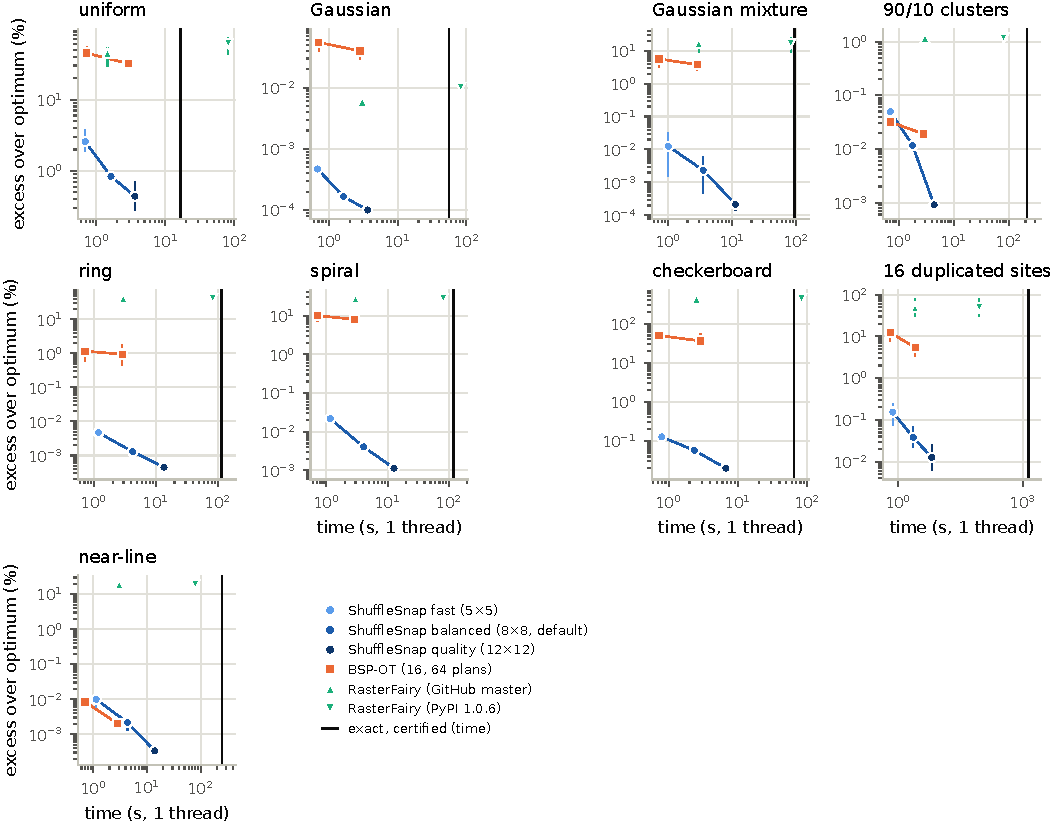
\includegraphics[width=\linewidth]{figures/fig_tradeoff_100k.pdf}
  \caption{Excess over the certified optimum against single-thread time at $N=100{,}000$
  (mean over three held-out instances; bars span min--max). The four \ShuffleSnap\ presets
  form the blue curve, from baseline to quality. BSP-OT at 16 and 64 plans is joined by an
  orange line. The black vertical line is the time of the certified exact solver.
  Heavy tails are omitted (all methods $<$0.001\%).}
  \label{fig:tradeoff}
\end{figure}

Table~\ref{tab:main} and Figure~\ref{fig:tradeoff} summarize the held-out comparison at
$10^5$ points on one thread.

\paragraph{\ShuffleSnap.} On nine of the eleven distributions, the baseline as specified
is within 0.2\% of the optimum, and on six of them within 0.03\%. It needs a median of
5\,s on one thread. The two exceptions are uniform points (2.5\%) and the jittered
lattice (33\%). There the optimum is small, so the long loops of
Section~\ref{sec:anatomy} dominate. The presets trade time for quality almost monotonically. The one exception is the
90/10 clusters, where fast is slightly worse than the baseline (0.034\% vs.\ 0.031\%). Balanced (median 16\,s) reduces the uniform excess to 0.84\%, and
quality (median 52\,s) to 0.44\%. The jittered lattice remains hard even for quality
(7.4\%): in absolute terms, 0.03 cells$^2$ per point against an optimum of 0.43
(Table~\ref{tab:abs}).

\paragraph{BSP-OT} is the fastest method (0.7\,s for 16 plans, 2.9\,s for 64). Its
excess, however, is typically 10--350$\times$ that of the \ShuffleSnap\ baseline:
32\% on uniform points, 36\% on the checkerboard, 8\% on the spiral and 3.7\% on the
mixture, all with 64 plans. It is competitive on two inputs. On the near-line, 64 plans
(0.002\%) match the balanced preset, and on the 90/10 clusters they beat the baseline
(0.019\% vs.\ 0.031\%) but not balanced (0.012\%).

\paragraph{RasterFairy (upstream)} takes about 3\,s. Its recursive slicing, however, costs
17--425\% on seven of the eleven distributions. It does well on three: the Gaussian
(0.006\%), the 90/10 clusters (1.2\%), and the jittered lattice, where it matches the
balanced preset (13.2\% vs.\ 12.7\%) because slicing a noisy lattice recovers the lattice.
The PyPI release, with pre-scaled inputs, gives similar or worse costs (e.g.\ 62\% vs.\ 45\%
on uniform points) and takes 80\,s at this size. Its targets at 50k and 100k points have a partially filled
last row, which sends it into its much slower mask code path; at $N=10^4$, a full
$100\times100$ square, it needs 0.03\,s.

\paragraph{With all cores.} On 24 hardware threads, \ShuffleSnap\ ran 13--15$\times$ faster than on
one and returned bit-identical assignments in all 396 paired runs. At $10^5$ points the
median time is 0.35\,s for the baseline, 1.1\,s for balanced and 3.9\,s for quality.
BSP-OT gained 4--7$\times$ (0.13\,s with 16 plans, 0.42\,s with 64); its plans are computed
in parallel, but the cycle-merging pass that combines them is largely sequential. At 24 threads, the baseline and BSP-OT with
64 plans therefore take about the same time, and the baseline has lower excess on nine of
the eleven distributions. The two exceptions are the near-line and the 90/10 clusters,
as above.

\paragraph{Exact solutions.} Started from \ShuffleSnap, the certified solver finished every
instance, in 7\,s (jittered lattice) to 23\,min (16 duplicated sites), with a median of
128\,s. That is 5--500$\times$ the time of the \ShuffleSnap\ baseline (median 25$\times$).
Started from bisection instead, it failed on four instances (mixture, duplicates,
near-line, spiral): no certificate within an hour or 50 pricing rounds. On six of the
seven instances where it did certify, it was 1.2--24$\times$ slower; on the jittered
lattice it was slightly faster (5\,s vs.\ 7\,s). The start matters because the candidate edges come from it:
\ShuffleSnap's layout is close enough to optimal that few pricing rounds are needed. A
dense exact solver is not an option at this size. Already at $N=10^4$, SciPy needed
3--352\,s (Table~\ref{tab:main10k} in the appendix), whereas the certified sparse solver
needed 0.3--7.7\,s.

\subsection{Quality at a matched time budget}
\label{sec:anytime}

\begin{figure}[tbp]
  \centering
  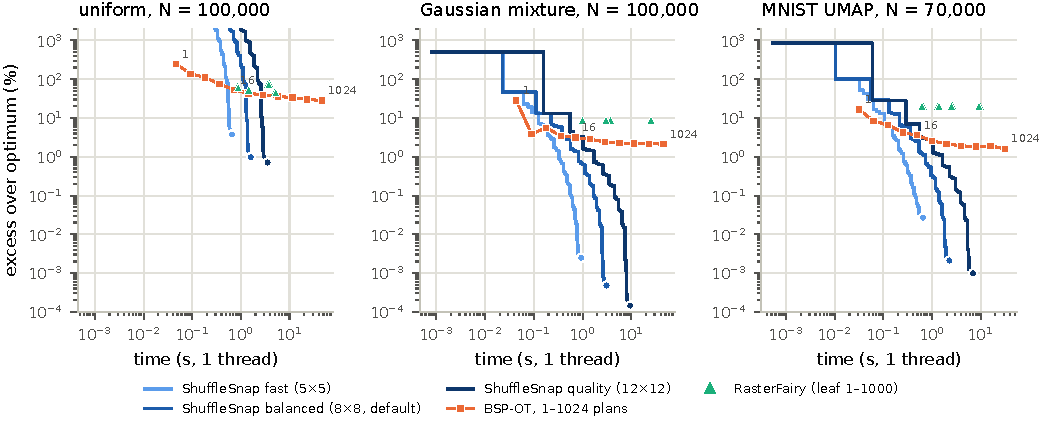
\includegraphics[width=\linewidth]{figures/fig_anytime_t1.pdf}
  \caption{Excess over the certified optimum against elapsed time, one thread. \ShuffleSnap's
  step curves record the exact cost after every phase, so each shows the result that a time
  budget ending at that moment would return. BSP-OT is run separately with 1, 2, 4, \dots,
  1024 plans (labels at 1, 16 and 1024). RasterFairy upstream is shown with exact leaf
  blocks of 1, 50, 200 and 1000 points. Instance seed 1. The same plot with 24 threads is
  in the appendix (Figure~\ref{fig:anytime24}).}
  \label{fig:anytime}
\end{figure}

Figure~\ref{fig:anytime} compares the methods at matched time budgets. BSP-OT improves
slowly with more plans and levels off far from the optimum. From 1 to 16 to 1024 plans,
its excess drops from 249\% to 53\% to 28\% on uniform points, from 28\% to 3.1\% to
2.1\% on the mixture, and from 16\% to 3.6\% to 1.6\% on MNIST. The 1024-plan runs take
31--46\,s on one thread. The \ShuffleSnap\ baseline passes that best BSP-OT result after
1.1--1.3\,s and finishes at 2.5\%, 0.004\% and 0.014\% respectively. At equal elapsed
time, \ShuffleSnap\ is ahead from 0.7--1.3\,s onward. With less time than that (on one
thread at $10^5$ points), BSP-OT is the better choice, because \ShuffleSnap\ has only
finished its coarsest levels. With 24 threads, the crossover moves to 0.04--0.09\,s.
RasterFairy's leaf size hardly matters except on uniform points (73\% with no exact leaves,
45\% with 1000-point leaves).

\subsection{Scaling in time and memory}
\label{sec:scaling}

\begin{figure}[tbp]
  \centering
  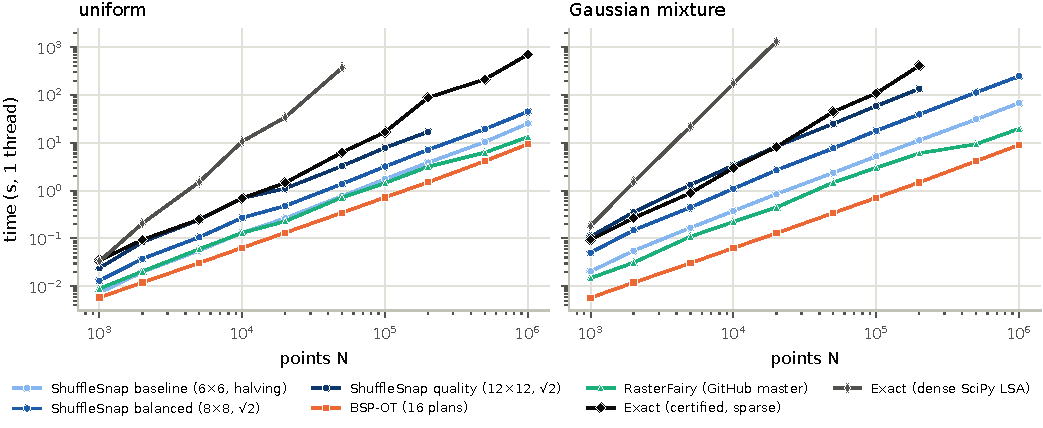
\includegraphics[width=\linewidth]{figures/fig_scaling.pdf}
  \caption{Time against $N$ on one thread (instance seed 1). Dense SciPy was run up to the
  largest size we considered sensible, 50k uniform points (6.2\,min, 23\,GiB) and 20k
  mixture points (22\,min). The certified solver was run up to $10^6$ uniform and
  $2\times10^5$ mixture points. The quality preset was run up to $2\times10^5$ points.}
  \label{fig:scaling}
\end{figure}

\begin{table}[tbp]
\centering\small
\caption{Peak extra resident memory (MiB) during one call, measured on a heap trimmed right
before the call (\texttt{malloc\_trim}), one thread, instance seed 1. Without trimming,
small allocations can reuse pages freed while the instance was generated and go unseen.}
\label{tab:memory}
\begin{tabular}{lrrrrrr}
\toprule
 & \multicolumn{3}{c}{uniform} & \multicolumn{3}{c}{Gaussian mixture} \\
method & $10^4$ & $10^5$ & $10^6$ & $10^4$ & $10^5$ & $10^6$ \\
\midrule
ShuffleSnap fast & 0.6 & 5.4 & 52.2 & 0.6 & 5.5 & 52.2 \\
ShuffleSnap balanced & 0.6 & 5.4 & 52.2 & 0.6 & 5.5 & 52.2 \\
ShuffleSnap quality & 0.6 & 5.4 & 52.2 & 0.6 & 5.5 & 52.2 \\
BSP-OT, 16 plans & 2.2 & 24.2 & 243 & 2.4 & 24.3 & 244 \\
RasterFairy master & 6.2 & 63.4 & 647 & 6.2 & 62.9 & 647 \\
exact, certified sparse & 49.5 & 437 & -- & 76.5 & 772 & -- \\
exact, dense SciPy & 1563 & -- & -- & 1564 & -- & -- \\
bisection only & 0.1 & 1.2 & 11.4 & 0.1 & 1.1 & 13.3 \\
\bottomrule
\end{tabular}

\end{table}

Between $10^4$ and $10^6$ points, \ShuffleSnap, BSP-OT and RasterFairy all scale close to
linearly. Their fitted exponents of time in $N$ are 1.15--1.18, 1.08 and about 1.0
(Figure~\ref{fig:scaling}). The time match with BSP-OT holds at $10^6$ uniform points: the fast
preset takes 9.8\,s on one core and BSP-OT with 16 plans 9.4\,s. The default takes 21\,s; with
24 threads, fast and default take 0.9\,s and 1.5\,s, and BSP-OT 2\,s. On the mixture, $10^6$
points take 14\,s (fast) and 43\,s (default) on one thread, or 1.0\,s and 2.7\,s on 24 threads.
RasterFairy takes 13--20\,s on one thread.

Exact solving scales worse but reaches further than we expected. The certified solver's
time grew as $N^{1.6}$ on uniform points and $N^{1.7}$ on the mixture. It certified $10^6$
uniform points in 11\,min using 4.2\,GiB, and $2\times10^5$ mixture points in 6.6\,min. Its
memory, 4--8\,kB per point, is set by the candidate edges and the flow solver. Dense SciPy
grew as $N^{2.2}$ (uniform) to $N^{2.9}$ (mixture) and needs $8N^2$ bytes. It took 6.2\,min
and 23\,GiB at 50k uniform points, and 22\,min at 20k mixture points. \ShuffleSnap\ needs
$O(N)$ working memory: an occupancy array, a position array, a last-change stamp per cell,
the window lists of the current level, and the input checks' temporary arrays. Measured,
this is 55--58 bytes per point at $10^5$ and $10^6$ points, or 52\,MiB at $10^6$
(Table~\ref{tab:memory}). The comparators need 4--12$\times$ more: BSP-OT about 250 and
RasterFairy about 670 bytes per point.

At $10^6$ uniform points, the quality ranking is unchanged. Measured against the certified
optimum of that instance, the excess is 3.3\% for fast, 1.3\% for the default and 0.58\% for
quality, against 74\% for BSP-OT (16 plans) and 48\% for RasterFairy. On uniform points the
default's excess grows with $N$: 0.11\% at $10^3$, 0.97\% at $10^5$ and 1.3\% at $10^6$ (one
instance each).

\paragraph{A billion points.} To see how far the method reaches beyond the benchmark, we solved
the largest instance of the earlier \ShuffleSnap\ work: 1{,}000{,}014{,}129 points of a 2D
random walk (the ``meander''), normalized to the unit square, on a $31{,}623\times31{,}623$
grid. We used the same random-permutation start, the default preset and 24 threads, on
the same workstation (Figure~\ref{fig:billion}). A dense cost matrix
would take 8\,EB. Setting up the start and the occupancy took 32\,s, and memory peaked at
53\,GiB, 57 bytes per point: coordinates and cell centers take 16 bytes each, change stamps
8, positions, occupancy and the grid index 4 each, and the window lists about 5. The kernel
accepts any mask; for a full rectangle, the centers and the index could be computed instead
of stored, which would save 20 of the 57 bytes. The walk is so concentrated that the result
moves the average point by about 6{,}900 cells (root mean square).

The default preset reached its fixed point after 1\,h\,43\,min (stride 1 began at
1\,h\,30\,min, and 78 stride-1 rounds followed). The coarse levels took about 4 minutes each,
because at this size nearly every window changes at every level and none can be skipped.
We then ran the quality preset's last four levels ($12\times12$ windows, strides 4 to 1),
which converged after 4.1\,h in total and lowered the cost by only $1.2\times10^{-6}$\%. Progress was front-loaded, as at smaller sizes: the cost
was within 1\% of the final one after 11 minutes, 0.1\% after 22, 0.01\% after 34 and 0.001\%
after 46, and after one hour it was only 0.0001\% above it.

No optimum is known for this instance, so we priced other assignments of the same instance on
the same frame. The earlier implementation ($6\times6$ windows, halving strides, 24 threads)
ran for six hours without converging. It reached stride 1 after 87 minutes and ended 0.0017\%
above our final cost, a level our run passed after 44 minutes. A memory-lean single-plan
port of BSP-OT, written for the earlier work because the official multi-plan code does not fit
in memory at this size, took 392\,s on one thread and is 8.2\% above. This is one instance
with no optimality certificate. It shows that the method runs to convergence at $10^9$ points
on one workstation, not how close it comes to the optimum there.

\begin{figure}[tbp]
  \centering
  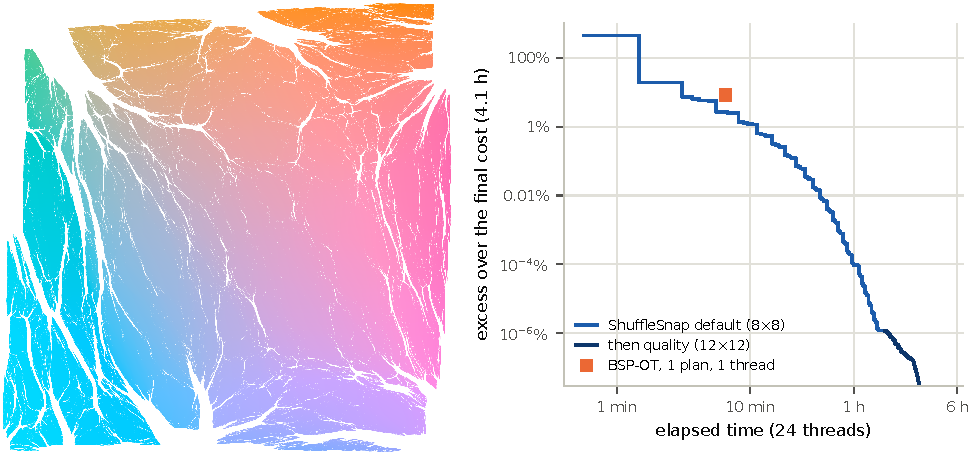
\includegraphics[width=\linewidth]{figures/fig_billion.pdf}
  \caption{A billion points. Left: every point drawn 75\% of the way from its
  input position to its assigned cell, one pixel per point, colored by input position and
  averaged over $10{,}000^2$ pixels (shown downsampled). White seams open where neighbouring
  cells hold points from distant sources; they follow the walk's folds. Right: cost after
  every phase as excess over the final cost: the default preset until its fixed point, then
  the quality preset's last four levels. A single-plan BSP-OT port is shown for comparison.}
  \label{fig:billion}
\end{figure}

\subsection{Real embeddings: displacement versus neighbourhoods}
\label{sec:real}

\begin{figure}[tbp]
  \centering
  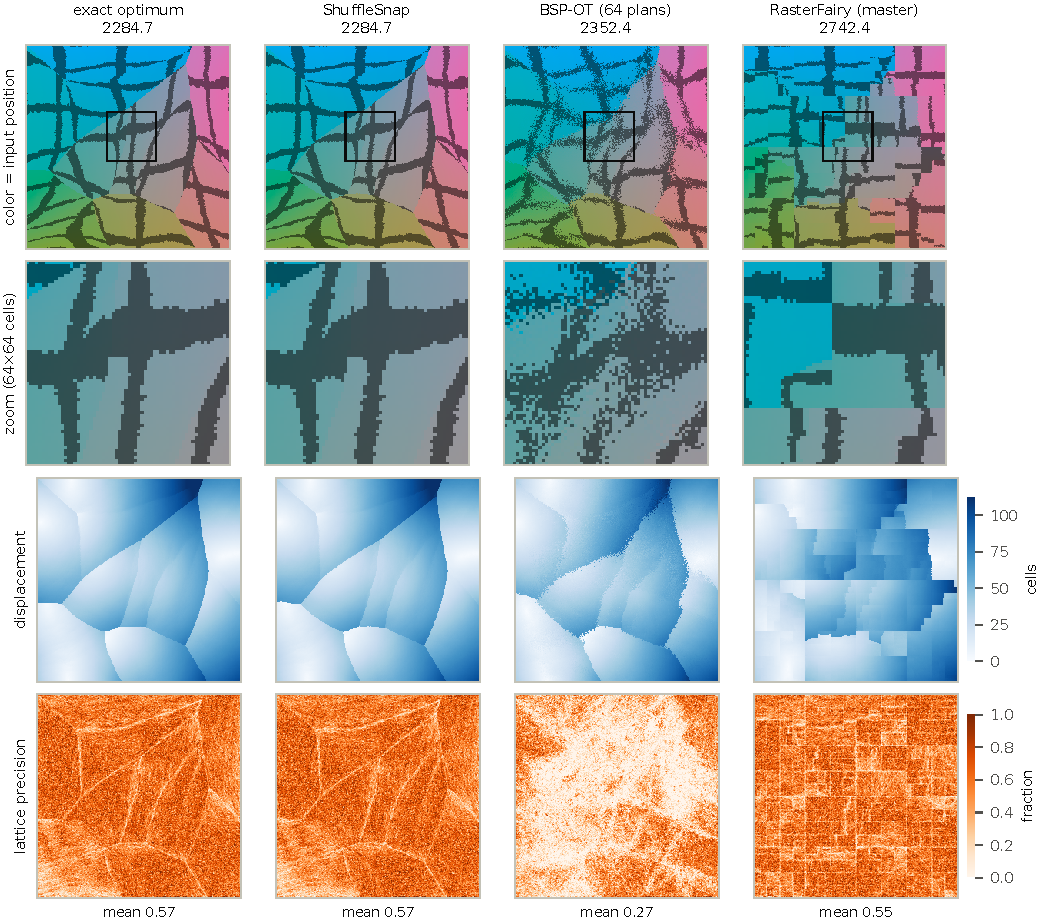
\includegraphics[width=\linewidth]{figures/fig_visual_mnist.pdf}
  \caption{All 70{,}000 MNIST digits, UMAP layout snapped to a $265\times265$ grid. Each
  point has the same color in every panel, set by its position in the input layout, and the
  dark bands are graph-paper lines drawn on the input, so bent lines show how a method
  deforms the layout, and color jumps or broken lines show where it tears it. The number under each method name is
  the mean squared displacement in cells$^2$. Row~2 enlarges the $64\times64$ box. Row~3
  shows each point's displacement. Row~4 shows the distance from each point's cell to its
  cell in the certified optimum (logarithmic scale; white means the optimal cell, so the
  optimum's own panel is blank). Row~5 shows lattice precision: the fraction of a
  point's occupied 8-neighbour cells whose points are among its 8 nearest input
  neighbours (higher is better). \ShuffleSnap\ is visually indistinguishable from the
  certified optimum: 74\% of its points sit on their optimal cell, and its few errors form
  the thin loops of one-cell shifts of Section~\ref{sec:anatomy}. BSP-OT is within 3\% of
  the optimal displacement, yet its median point is 8 cells from its optimal cell, and it
  halves lattice precision, because it scrambles local order (frayed lines and speckled
  boundaries in rows~1--2). RasterFairy's recursive slicing breaks the lines at rectangular seams.}
  \label{fig:visual}
\end{figure}

\begin{table}[tbp]
\centering\scriptsize
\setlength{\tabcolsep}{3.5pt}
\caption{Real embeddings, all 70{,}000 points (square exact-fit grid). Excess over the
certified optimum and neighbourhood measures are means over three method seeds; times are
medians on one thread (1T) and on 24 threads (24T, methods that use threads only). Memory is
the rise of peak resident memory during the call. kNN recall: fraction of each point's 10
nearest input neighbours among its 10 nearest grid neighbours. Lattice precision: fraction
of occupied 8-neighbour cells holding one of the point's 8 nearest input neighbours.}
\label{tab:real}
\resizebox{\linewidth}{!}{\begin{tabular}{llrrrrrrr}
\toprule
 & method & excess (\%) & mean sq. & time 1T (s) & time 24T (s) & mem (MiB) & kNN recall & lattice prec. \\
\midrule
MNIST UMAP & exact (certified) & 0 & 2284.7 & 82.0 & -- & 562 & 0.645 & 0.581 \\
 & ShuffleSnap fast & 0.031 & 2285.4 & 0.66 & 0.064 & 2 & 0.644 & 0.578 \\
 & ShuffleSnap balanced & 0.002 & 2284.7 & 2.27 & 0.16 & 2 & 0.645 & 0.580 \\
 & ShuffleSnap quality & $<$0.001 & 2284.7 & 7.03 & 0.54 & 2 & 0.644 & 0.580 \\
 & BSP-OT, 16 plans & 3.73 & 2370.0 & 0.49 & 0.088 & 16 & 0.305 & 0.255 \\
 & BSP-OT, 64 plans & 2.42 & 2340.0 & 1.98 & 0.28 & 42 & 0.305 & 0.249 \\
 & RasterFairy master & 20.0 & 2742.4 & 1.38 & -- & 42 & 0.631 & 0.551 \\
 & RasterFairy PyPI & 44.5 & 3301.0 & 11.2 & -- & 44 & 0.602 & 0.534 \\
 & bisection only & 34.4 & 3071.1 & 0.023 & -- & 0 & 0.569 & 0.498 \\
\addlinespace
Fashion UMAP & exact (certified) & 0 & 1802.6 & 76.0 & -- & 566 & 0.606 & 0.548 \\
 & ShuffleSnap fast & 0.008 & 1802.7 & 0.67 & 0.056 & 2 & 0.606 & 0.548 \\
 & ShuffleSnap balanced & 0.001 & 1802.6 & 2.31 & 0.17 & 2 & 0.607 & 0.547 \\
 & ShuffleSnap quality & $<$0.001 & 1802.6 & 7.23 & 0.56 & 2 & 0.607 & 0.547 \\
 & BSP-OT, 16 plans & 9.15 & 1967.5 & 0.50 & 0.088 & 16 & 0.295 & 0.245 \\
 & BSP-OT, 64 plans & 6.73 & 1923.8 & 1.98 & 0.28 & 42 & 0.334 & 0.275 \\
 & RasterFairy master & 24.6 & 2245.3 & 1.38 & -- & 42 & 0.611 & 0.532 \\
 & RasterFairy PyPI & 25.6 & 2264.5 & 11.1 & -- & 44 & 0.594 & 0.526 \\
 & bisection only & 23.0 & 2217.7 & 0.023 & -- & 0 & 0.544 & 0.477 \\
\bottomrule
\end{tabular}
}
\end{table}

Figure~\ref{fig:visual} and Table~\ref{tab:real} compare the methods on the full MNIST
and Fashion-MNIST embeddings. The default preset is within 0.002\% of the certified
optimum on both datasets, and the fast preset within 0.031\%. At about the same time as BSP-OT
with 16 plans (0.66\,s against 0.49\,s on one core), the fast preset is at 0.031\% and
0.008\%, where BSP-OT is at 3.7\% and 9.2\%.
In every panel their colour fields match the optimum's.

The two measures disagree on BSP-OT. With 64 plans, its displacement is only 2.4\% (MNIST) and
6.7\% (Fashion) above optimal, yet both neighbourhood measures fall to about half: kNN recall
0.31--0.33 against 0.61--0.65 for the optimum, and lattice precision 0.25--0.28 against
0.55--0.58. Averaged over plans, the merged BSP partitions are close to the transport
map, but they shuffle points locally. RasterFairy shows the opposite pattern: its
displacement is 20--25\% above optimal, yet its neighbourhood measures are close to the
optimum's. On Fashion-MNIST its kNN recall (0.611) even exceeds the optimum's (0.606),
because local order survives inside each slice and breaks only along the seams.
\ShuffleSnap's measures match the optimum's to within 0.003. Compared cell by cell with the
optimum (row~4, the figure's runs), \ShuffleSnap\ leaves 74\% (MNIST) and 69\% (Fashion)
of the points on their optimal cell and 93\% and 91\% within one cell, while BSP-OT's and
RasterFairy's median points are 8 and 19 cells from theirs on both embeddings. Even the optimum has lattice precision well below 1: an optimal transport map
from clustered data to a uniform grid tears the layout along cluster boundaries (the
white lines in row~5). Minimizing displacement and preserving neighbourhoods are
different objectives, and neither implies the other.

\subsection{Masks, surplus cells and prime counts}
\label{sec:masks}

\begin{figure}[tbp]
  \centering
  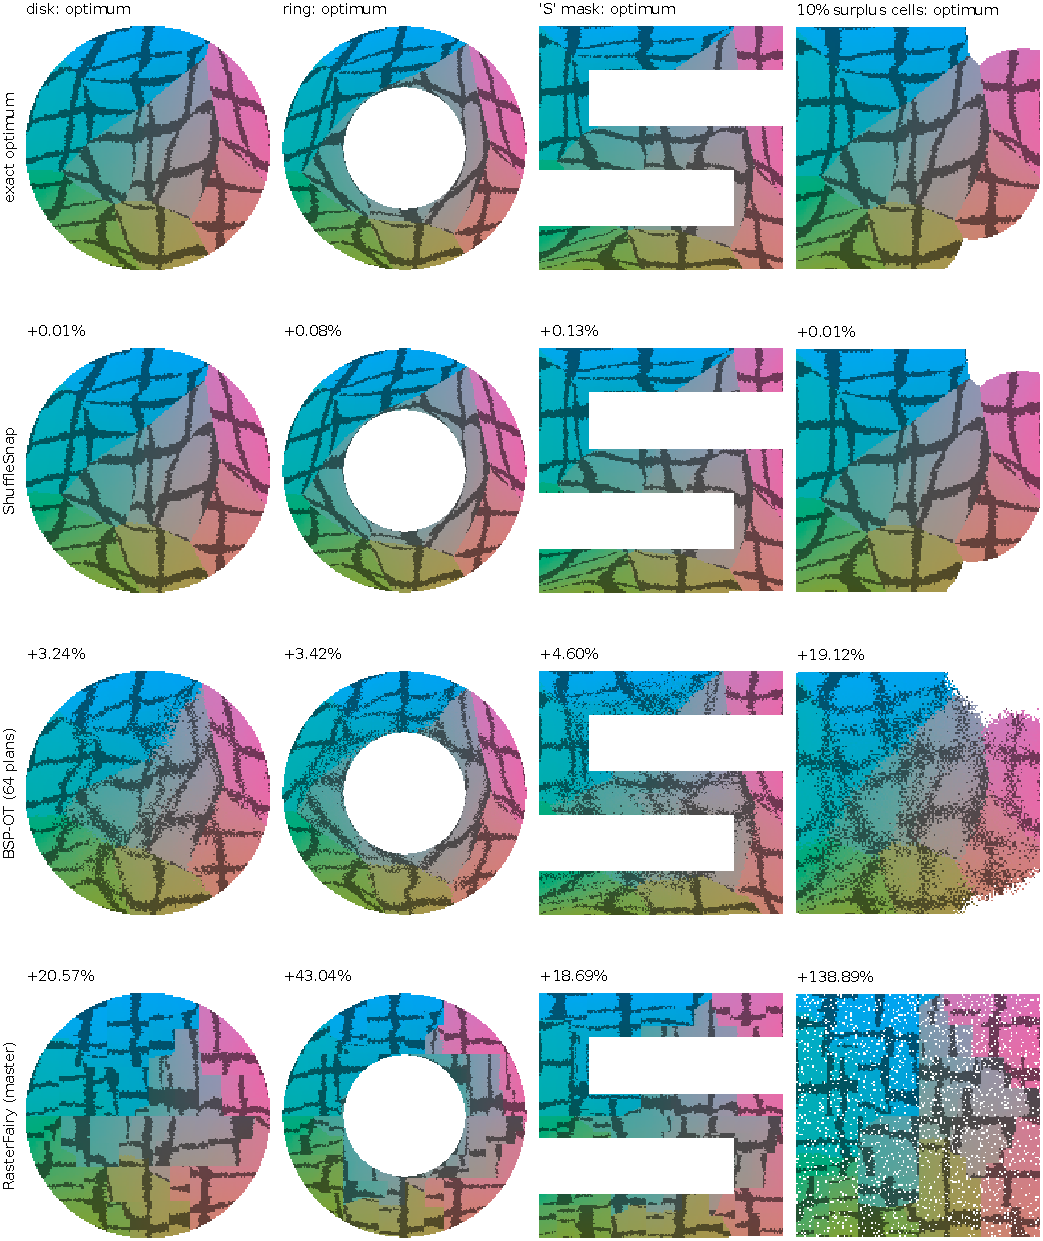
\includegraphics[width=\linewidth]{figures/fig_masks.pdf}
  \caption{A 20{,}000-point subset of the MNIST UMAP embedding on a disk, a ring, an
  S-shaped mask, and a rectangle with 10\% surplus cells (instance seed 1; colors encode
  input position as in Figure~\ref{fig:visual}; white = empty or masked). Numbers are
  excess over the certified optimum. With surplus cells, the optimum leaves one contiguous
  region empty, far from the data, and \ShuffleSnap-balanced finds the same region.
  BSP-OT's partial matching leaves ragged holes along the boundary, and RasterFairy
  removes surplus cells at random before slicing.}
  \label{fig:masks}
\end{figure}

\begin{table}[tbp]
\centering\scriptsize
\setlength{\tabcolsep}{3.5pt}
\caption{Excess over the certified optimum (\%) on non-square targets, $N=20{,}000$, mean of
instance seeds 1--3 (all 24 exact runs certified). ``Surplus ($<$1 row)'' is the full
$W\times H$ rectangle holding $N$ points, with fewer than $W$ empty cells;
``10\% surplus'' has $1.1N$ cells.}
\label{tab:masks}
\resizebox{\linewidth}{!}{\begin{tabular}{llrrrrrr}
\toprule
target & points & SS fast & BSP 16 & SS bal. & BSP 64 & SS qual. & RF master \\
\midrule
surplus ($<$1 row) & uniform & 6.31 & 90.3 & 3.10 & 85.0 & 1.37 & 56.6 \\
surplus ($<$1 row) & Gaussian mixture & 0.033 & 8.41 & 0.013 & 7.95 & 0.010 & 17.2 \\
surplus ($<$1 row) & spiral & 0.099 & 19.9 & 0.006 & 11.5 & 0.003 & 32.4 \\
surplus ($<$1 row) & MNIST UMAP & 0.082 & 16.5 & 0.020 & 5.29 & 0.011 & 43.6 \\
\addlinespace
10\% surplus & uniform & 3.81 & 108.9 & 0.91 & 58.7 & 0.25 & 350.5 \\
10\% surplus & Gaussian mixture & 0.43 & 30.5 & 0.055 & 17.6 & 0.012 & 71.6 \\
10\% surplus & spiral & 0.61 & 26.2 & 0.071 & 19.3 & 0.012 & 157.9 \\
10\% surplus & MNIST UMAP & 0.077 & 29.4 & 0.007 & 22.8 & 0.003 & 146.2 \\
\addlinespace
4:1 rectangle & uniform & 2.64 & 32.3 & 1.34 & 23.9 & 0.45 & 26.4 \\
4:1 rectangle & Gaussian mixture & 0.23 & 1.44 & 0.024 & 0.81 & 0.004 & 6.70 \\
4:1 rectangle & spiral & 0.34 & 4.33 & 0.067 & 2.34 & 0.022 & 15.4 \\
4:1 rectangle & MNIST UMAP & 0.18 & 2.07 & 0.014 & 1.28 & 0.003 & 11.6 \\
\addlinespace
disk & uniform & 0.034 & 8.64 & 0.014 & 6.74 & 0.006 & 11.4 \\
disk & Gaussian mixture & 0.016 & 5.43 & 0.003 & 4.27 & $<$0.001 & 37.0 \\
disk & spiral & 0.024 & 5.19 & 0.007 & 2.48 & 0.003 & 23.6 \\
disk & MNIST UMAP & 0.022 & 4.49 & 0.006 & 2.77 & 0.002 & 20.3 \\
\addlinespace
ring & uniform & 0.067 & 9.28 & 0.028 & 6.73 & 0.006 & 53.6 \\
ring & Gaussian mixture & 0.11 & 6.75 & 0.048 & 4.81 & 0.018 & 35.9 \\
ring & spiral & 0.048 & 7.73 & 0.014 & 3.83 & 0.016 & 47.9 \\
ring & MNIST UMAP & 0.14 & 4.77 & 0.070 & 3.11 & 0.025 & 43.2 \\
\addlinespace
S mask & uniform & 16.6 & 12.1 & 1.43 & 9.30 & 0.88 & 60.8 \\
S mask & Gaussian mixture & 0.63 & 4.11 & 0.057 & 2.99 & 0.036 & 32.4 \\
S mask & spiral & 3.27 & 12.5 & 0.26 & 4.79 & 0.19 & 56.8 \\
S mask & MNIST UMAP & 1.55 & 6.23 & 0.12 & 4.53 & 0.093 & 19.0 \\
\bottomrule
\end{tabular}
}
\end{table}

Table~\ref{tab:masks} and Figure~\ref{fig:masks} cover non-square targets.
\begin{itemize}
\item \textbf{Convex masks.} On disks and rings, every \ShuffleSnap\ preset stays within
  0.25\% (baseline) and 0.07\% (balanced) of the optimum. BSP-OT is at 2.5--9\% and
  RasterFairy at 11--54\%.
\item \textbf{The S-shaped mask.} This is the baseline's worst case. With uniform points
  it is 18.3\% above optimal, worse than BSP-OT with 64 plans (13.2\%); with the spiral it
  is 7.3\%. The mechanism is the one in Figure~\ref{fig:failures}: coarse strides route
  mass across the bays. The $\sqrt2$ schedule repairs most of this. Balanced reaches
  1.3\% and 0.26\%, and quality 0.13\% and 0.04\%.
\item \textbf{Surplus cells.} When the solver must also choose the empty cells, the baseline
  degrades noticeably: 0.7--4.4\% with 10\% surplus, and 8.4\% for uniform points with
  less than one row of surplus. Balanced stays below 1\% everywhere except that last
  case (3.1\%), and quality stays below 1.4\%. Surplus is where the comparators suffer
  most. With 10\% surplus, BSP-OT's partial matching is 18--109\% above optimal, and
  RasterFairy, which picks the empty cells at random, is 72--350\% above optimal. With
  less than one row of surplus, they are at 5--90\% and 17--57\%.
\end{itemize}

\subsection{Ablations on held-out instances}
\label{sec:ablation}

\begin{figure}[tbp]
  \centering
  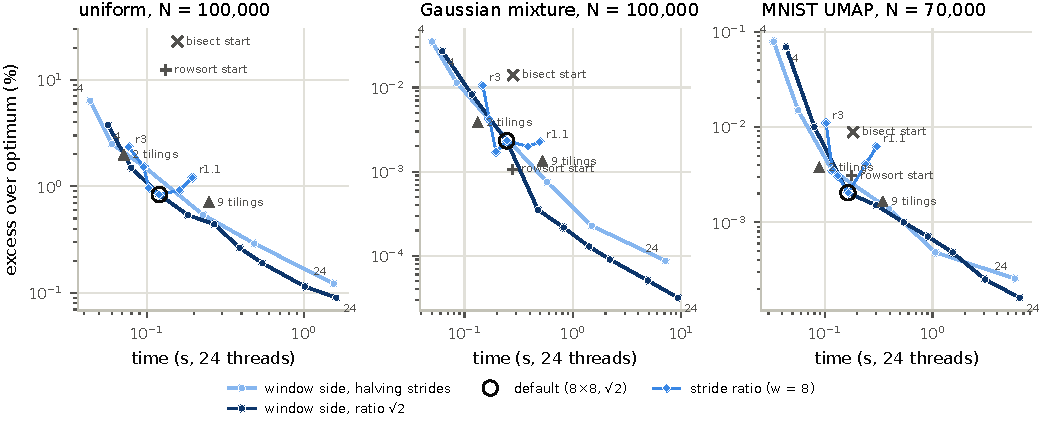
\includegraphics[width=\linewidth]{figures/fig_ablation.pdf}
  \caption{Held-out ablations. Each panel shows mean excess over the certified optimum against
  median time (24 threads, three instance seeds). Lines vary an ordered setting of the
  baseline: the window side, with halving (light) or $\sqrt2$ strides (dark), labelled
  by the side length; and the stride ratio at $w=6$ (diamonds; r3 and r1.1 mark the
  extremes). Markers show categorical changes to the baseline: bisection or row-sort
  starts, and 2 or 9 shifted tilings per round instead of 4. A single tiling
  ($>$20{,}000\% on uniform points) is off the chart. Solver choice and skipping unchanged
  windows do not change quality; they are listed with all other numbers in
  Table~\ref{tab:ablation}.}
  \label{fig:ablation}
\end{figure}

Figure~\ref{fig:ablation} varies one design choice at a time, starting from the baseline,
on instances that were not used for any design decision.
\begin{itemize}
\item \textbf{Window side} is the main quality knob. With halving strides, uniform
  excess falls from 15.7\% ($3\times3$) to 2.5\% ($6\times6$), 0.54\% ($12\times12$) and
  0.29\% ($16\times16$). Time rises from 0.05\,s to 1.5\,s on uniform points and from
  0.07\,s to 8.4\,s on the mixture. The $\sqrt2$ schedule shifts the whole curve down
  (e.g.\ 1.5\% at $6\times6$).
\item \textbf{Stride ratio}. $\sqrt2$ is best or close to best on all three inputs: on
  uniform points 1.5\% against 2.5\% for halving and 4.1\% for a ratio of 3, and 1.9\%
  for the finest ratio tested, 1.1. Finer is not always better.
\item \textbf{Coarse levels are essential}. Capping the first stride at 16, 8, 4, 2 or 1 (the
  last means stride-1 windows only, from the random start) made results 5--37$\times$
  worse and 5--90$\times$ slower. With halving from the automatic first stride of 64,
  uniform excess is 2.5\% in 0.12\,s; capped at 16 it is 11.7\% in 0.57\,s, and with
  stride 1 only it is 27\% in 1.3\,s. Without long-range moves, stride-1 windows need many
  rounds to repair a random start, and they stall far from the optimum.
\item \textbf{Start}. A random start beats bisection and row sorting by 4--18$\times$ (uniform:
  2.5\% against 29.9\% and 22.9\%). Better-looking starts contain straight seams that
  windows cannot undo.
\item \textbf{Shifted tilings are essential}. With a single fixed tiling, points can never
  cross a window border, and the method fails (uniform: excess over 20{,}000\%). Two
  diagonal shifts give 5.5\%, the four of the baseline 2.5\%, and nine shifts 1.9\% at
  twice the time. More rounds per level help about as much per second as larger windows
  (two rounds: 2.1\% at 1.4$\times$ the time).
\item \textbf{Window solver}. All three solvers are exact, so the assignments are
  identical. Jonker--Volgenant is 2--10$\times$ slower than the Hungarian method. The
  greedy warm start saves up to 15\% on uniform inputs but is 2--3\% slower on the
  clustered ones, so its benefit in the micro-benchmark (5--20\%) does not carry over
  consistently.
\item \textbf{Skipping unchanged windows} leaves results unchanged and saves 35--40\% of the time.
\item \textbf{Post-processing does not pay.} Three extra cycles of stride-2 and stride-1
  rounds after convergence changed nothing on uniform points and removed under 3\% of the
  excess on the clustered inputs. Merging four independent baseline runs, keeping the
  cheaper of the two assignments on every connected component of their union (the rule
  BSP-OT uses to merge plans), cut the uniform excess by 23--38\% at four times the cost.
  The fast preset does better (1.5\%) at about the same cost as the baseline on these
  uniform instances.
\end{itemize}

\subsection{Anatomy of the remaining error}
\label{sec:anatomy}

\begin{figure}[tbp]
  \centering
  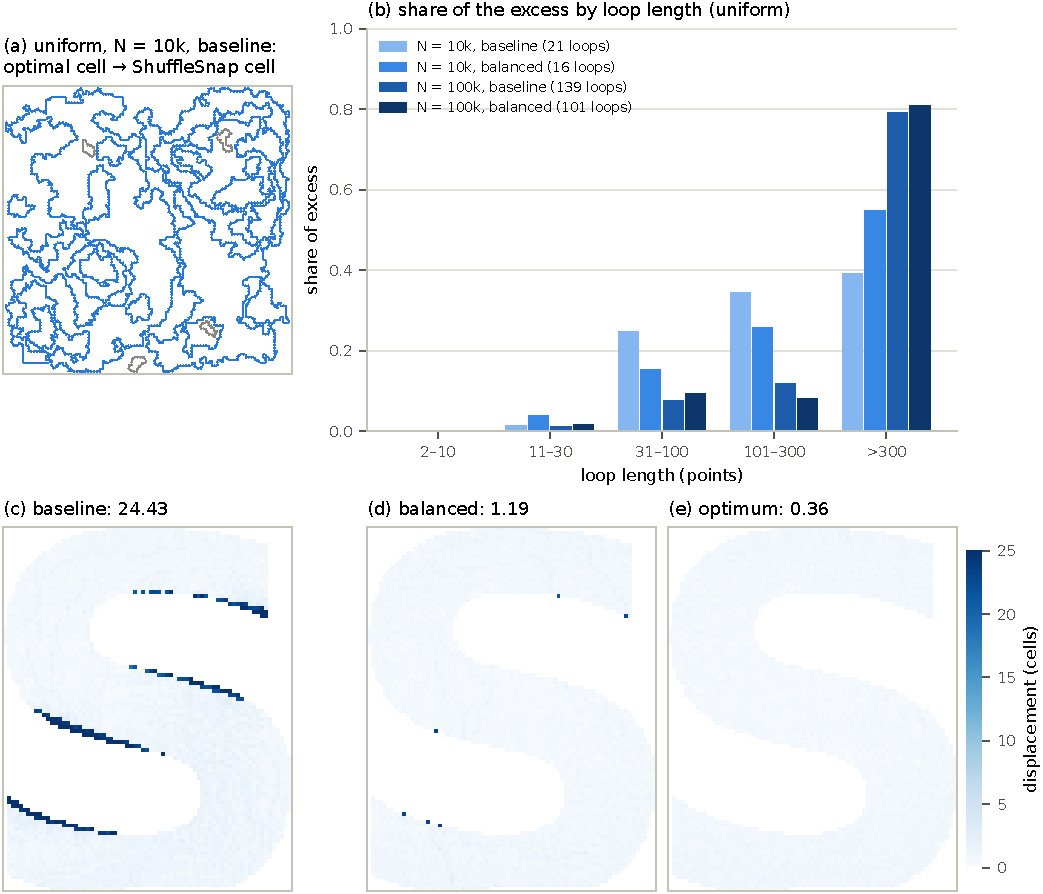
\includegraphics[width=\linewidth]{figures/fig_failures.pdf}
  \caption{Where \ShuffleSnap\ loses to the optimum (development instances, shown for
  mechanism rather than as claims). (a)~10{,}000 uniform points, default preset. Each arrow goes
  from a point's optimal cell to its \ShuffleSnap\ cell. The two layouts differ by closed
  loops of one-cell moves; loops longer than 30 points are blue. (b)~Share of the excess
  carried by loops of each length, for the fast and default presets: at $10^5$ points, about
  80\% of it sits in loops of more than 300 points. (c--e)~4{,}000 points drawn uniformly
  inside the rectilinear S-shaped mask, so that the optimum moves every point by less than a
  cell. With $6\times6$ windows and halving strides, points are routed across the concave bays
  and end up in long lines along their edges; the default preset leaves fewer such lines. Numbers are mean squared displacement.}
  \label{fig:failures}
\end{figure}

Why does a method that solves every window exactly still miss the optimum on uniform
data, by 0.84\% at $10^5$ points? Compare a \ShuffleSnap\ layout with the certified optimum. The
permutation that turns one into the other splits into cycles
(Figure~\ref{fig:failures}a). Almost all the excess sits in a handful of very long
cycles, in which every point is shifted by about one cell, so the layout is locally
rotated along a closed curve (Figure~\ref{fig:failures}b). Such a loop is invisible to
every window:
\begin{itemize}
\item Inside a stride-1 window, the part of a loop is a run of points shifted
  consistently by one cell, which is already the best arrangement of that occupant set.
  Undoing the loop requires moving one point out at one end of the run and one in at
  the other end.
\item Coarser windows cannot help either. A one-cell shift moves a point to another
  residue class, and a strided window only permutes points within one class.
\end{itemize}
Indeed, three extra cycles of stride-2 and stride-1 rounds after convergence changed
nothing on held-out uniform instances.

\paragraph{A constructed fixed point.} The argument can be checked directly. Put the
points exactly on the cell centers of a $64\times48$ grid, so that the optimum is the
identity with cost 0. Then rotate an axis-aligned ring of cells by one step: the point of
each ring cell moves to the next ring cell, so the cost equals the number $L$ of ring
cells. We ran the complete $\sqrt2$ schedule from this layout, with every stride and
every tiling, followed by stride-1 rounds to convergence. For windows of side
$w\in\{5,6,8,12,16\}$, a ring larger than the window was never touched (0 points moved), so
the result has cost $L$ against an optimum of 0. A ring of side at most $w/2+1$ always
lies inside one of the four shifted tilings and was repaired. A $6\times6$ ring
survived $6\times6$ windows when it straddled the borders of all four tilings. Relative
excess over the optimum is therefore unbounded for this method, and the package's test
suite includes this configuration as a documented limitation.

On real inputs, larger windows remove the shorter loops, and the $\sqrt2$ schedule creates
fewer loops in the first place, but the long loops remain: at $10^5$ uniform points, loops of
more than 300 points carry about 80\% of the default's excess (Figure~\ref{fig:failures}b).
Their number and total length grow with $N$, which is why the default's excess on
uniform points grows from 0.1\% at $10^3$ points to 0.84\% at $10^5$ and 1.3\% at $10^6$
(Section~\ref{sec:scaling}).

Masks make the same mechanism visible at a larger scale (Figure~\ref{fig:failures}c--e).
At a coarse stride, a window's cells can lie on both sides of a concave bay, so mass
gets routed across the bay. By the time the stride is 1, fixing the routing would
require moving a whole arm's worth of points along the arm, which no window can do.
On points drawn uniformly inside the S, where the optimum costs 0.17 cells$^2$ per point, $6\times6$
windows with halving strides ended at 32 cells$^2$ per point, with the misrouted points lined up
along the bays. The default's larger windows and finer $\sqrt2$ schedule revisit
intermediate scales and reduce the error (6.3 cells$^2$ per point) but do not remove it; the
held-out numbers are in Section~\ref{sec:masks}.

A mask can also cut exchanges off entirely. Two usable cells trade occupants only if some
scheduled window contains both. On a one-row mask whose only usable columns are 0 and 9,
stride 2 puts the two cells in different residue classes, and an 8-wide stride-1 window never
holds both. A swapped pair therefore stays swapped under the default preset, at any number of
rounds. The quality preset's 12-wide windows happen to repair this example, but not the
general problem: a mask guarantees a valid layout, not reach. The package's tests include
this case.

\subsection{Parallel scaling}
\label{sec:threads}

\begin{figure}[tbp]
  \centering
  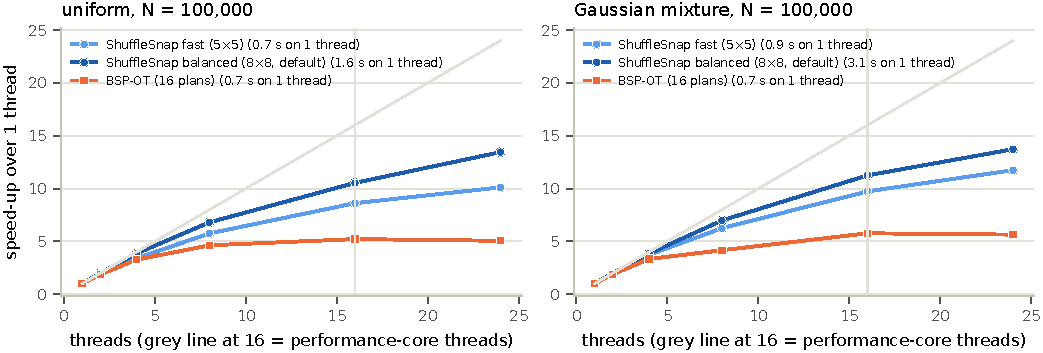
\includegraphics[width=\linewidth]{figures/fig_threads.pdf}
  \caption{Speed-up over one thread at $N=100{,}000$ (median of one run per setting,
  threads not pinned). The machine has 16 performance-core and 8 efficiency-core hardware
  threads; the light diagonal is linear speed-up. \ShuffleSnap's windows are independent
  within a phase, so it keeps scaling with the efficiency cores. BSP-OT stops improving
  at 8--16 threads, because its plans run in parallel but the merge that combines them is
  largely sequential.}
  \label{fig:threads}
\end{figure}

Figure~\ref{fig:threads} shows parallel scaling. \ShuffleSnap\ doubles its speed with each
doubling of threads up to 8 (7.7$\times$ at 8 threads). It reaches 12.5$\times$ at 16 and
14.8$\times$ at 24, with the same assignment at every thread count. BSP-OT reaches about
5--6$\times$ at 16 threads and gains nothing from the efficiency cores. We did not profile
where \ShuffleSnap\ loses efficiency beyond 8 threads. The efficiency cores are slower than
the performance cores, and each phase ends with a synchronization point.


\section{Discussion and limitations}
\label{sec:discussion}

\paragraph{What the hypothesis survived.} Coarse-to-fine strided windows get very close
to the optimum for the smooth, clustered layouts that motivate the problem. On the two
real 70{,}000-point UMAP embeddings, the default preset is within \RealBalancedExcess\ of
the certified optimum and visually indistinguishable from it. The method needs no dense
matrix, runs in 0.2--1.4\,s with all 24 threads at $10^5$ points (balanced preset), gives the same result for
any number of threads, and never increases the cost.

\paragraph{What it did not survive.} \ShuffleSnap\ is a local search, and its failures
follow from that. (i)~On near-uniform data, its relative excess grows with $N$ (for the
baseline, from about 1\% at $10^3$ points to 2.5\% at $10^5$ and 5.3\% at $10^6$). The excess consists of a
few long closed loops of one-cell shifts that no window can see whole. (ii)~Masks with
concave bays and grids with surplus cells need global rerouting of mass, which the
baseline gets wrong. With uniform points on the S-shaped mask it was 18\% above optimal,
worse than BSP-OT. The $\sqrt2$ schedule removes most of this (1.3\% for balanced, 0.13\%
for quality), but not all of it. (iii)~A good start does not help,
and structured starts hurt. (iv)~On a jittered lattice, where the optimum is almost the
identity, every heuristic we tested stays far from optimal in relative terms.

\paragraph{The exact solver changes the question.} We built the certified solver as an
evaluation tool. It turned out to be practical. Starting from \ShuffleSnap's answer, it proved optimality
at $10^5$ points in 7\,s to 23\,min on one core (median about 2\,min), and at $10^6$
uniform points in 12\,min.
When a certified optimum is worth the wait, it is the better choice at this scale, and
\ShuffleSnap's role is then that of a fast, good-enough answer, a warm start, and a
method for sizes and time budgets where exact solving is out of reach. We report this
even though it narrows the case for the method we set out to test.

\paragraph{Displacement is not neighbourhood.} BSP-OT reaches within a few percent of the
optimal displacement on the real embeddings, but halves the fraction of lattice
neighbours that were input neighbours, because merging many partitions shuffles points
locally. RasterFairy keeps local order inside its blocks and breaks it along block seams.
If neighbourhood preservation is the goal, it should be optimized directly (e.g.\ with
LAS/FLAS~\citep{barthel2023improved}); minimizing displacement buys it only to the
extent that the optimal transport map is smooth.

\paragraph{Limitations of this study.} Everything ran on one workstation, CPU only.
BSP-OT has a CUDA implementation that we did not test. The objective is squared
Euclidean displacement in 2D. The window solver works for any cost, but we did not
evaluate other costs or 3D grids. The certified solver depends on OR-Tools and on
integer scaling. Its certificate accounts for the scaling, but its running time depends
on the candidate set and the warm start. Real data consist of two UMAP embeddings with
one parameter setting. The bbox normalization is part of the problem definition; other
normalizations change the optimum. Timings include warm-up exclusions and a fixed
pinning policy, and unrelated background services were running (load about 1). We
compared against the representative settings of each comparator, but not every setting.
In particular, RasterFairy's swap optimizer was excluded because it requires dense
$N\times N$ memory and does not run on Python~3 as released.


\bibliographystyle{plainnat}
\bibliography{refs}

\appendix
\section{Reproducing the results}
\label{app:repro}

The paper repository (\href{https://github.com/kylemcdonald/shufflesnap-paper}{\nolinkurl{github.com/kylemcdonald/shufflesnap-paper}}) contains every script, raw result, and figure
source. The implementation is a separate repository (\href{https://github.com/kylemcdonald/shufflesnap}{\nolinkurl{github.com/kylemcdonald/shufflesnap}}); the benchmarked code is
identical, apart from its version string, to release 0.4.0 on PyPI
(\texttt{pip install shufflesnap}). Starting from a checkout of both side by side:
{\small
\begin{verbatim}
pip install ./shufflesnap[exact]   # C++ build, ~2 s
pip install -r shufflesnap-paper/requirements.txt
cd shufflesnap-paper
python experiments/make_embeddings.py mnist fashion   # UMAP, fixed seed
python experiments/references_all.py 6                # certified optima (parallel)
bash experiments/make_frozen_snapshot.sh              # v0.4.0 snapshot under test
bash experiments/run_all.sh                           # all benchmarks, sequential
bash experiments/run_swap.sh                          # RasterFairy's swap optimizer
python experiments/small_exactness.py                 # small-N exactness table
python experiments/dev_ablation.py                    # development-set search
python experiments/seed_study.py                      # spread over inputs and starts
python experiments/seed_study_report.py
python experiments/make_figures.py all && python experiments/make_tables.py
python experiments/fig_method.py; python experiments/fig_failures.py
python experiments/fig_reference.py                   # annotated reference
python experiments/fig_visual.py mnist; python experiments/fig_visual.py fashion
python experiments/fig_masks.py
cd paper && tectonic main.tex
\end{verbatim}
}
Raw results are JSON lines in \texttt{results/raw/}: one record per run, holding the
full run specification, timings, memory, validity check, cost, displacement statistics,
and the software environment (library versions, commit hashes of the comparator
repositories). Certified optima are cached in \texttt{results/reference/} with their
lower bound and gap. The lab notebook \texttt{notebook/LOG.md} records decisions and
negative results in the order they happened.

\paragraph{Timing boundary (summary).} A timed run is one call of a method adapter in a fresh
process, after a warm-up call on a 256-point instance. It includes method-specific
preprocessing and excludes instance generation, the shared normalization, and
validation. Peak memory is the rise of peak RSS during the call.

% Generated by experiments/fig_reference.py from paper/reference.py; do not edit.
\begin{landscape}
\section{A serial reference implementation}
\label{app:reference}

\noindent\begin{minipage}[t]{0.405\linewidth}\vspace{0pt}\raggedright
{\small This is the complete algorithm: the file \texttt{shufflesnap/reference.py} from the
package, split into its parts, each beside a diagram computed with its code. Without exact
ties it returns the same assignment as the compiled kernel; the package's tests check this
for every preset on six kinds of target, from an exact-fit square to surplus cells and a
random mask. The kernel adds threads, skips windows whose cells have not changed (which does
not change the result) and an optional time budget. Points are in grid units: cell $(x,y)$
has its center at $(x,y)$.\par}
\end{minipage}\hfill
\begin{minipage}[t]{0.565\linewidth}\vspace{0pt}
\lstinputlisting[firstline=1,lastline=12,firstnumber=1,numbers=left,numberstyle=\tiny\color{black!45},numbersep=6pt,frame=none,xleftmargin=1.6em,aboveskip=0pt,belowskip=0pt]{reference.py}
\end{minipage}

\vspace{1.4em}
\noindent\begin{minipage}[t]{0.405\linewidth}\vspace{0pt}\raggedright
\textbf{The schedule.}\par\smallskip
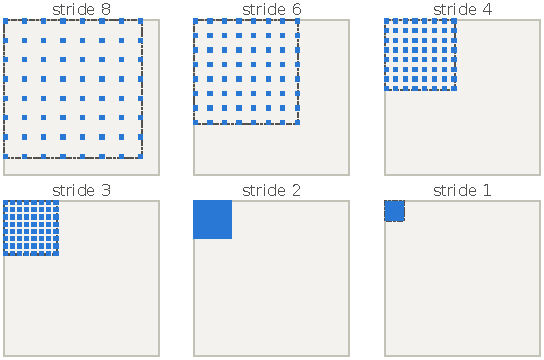
\includegraphics[width=\linewidth]{figures/fig_ref_schedule}\par\smallskip
{\small A window always holds $w\times w$ cells, but at stride $s$ they lie $s$ cells apart, so
it spans $(w-1)s+1$ cells per axis (dashed). The first stride is the smallest power of two
with $ws\ge L$, so the first windows reach across the axis; each later stride is the last one
divided by \texttt{ratio} and rounded. Each axis has its own strides, and the shorter axis
waits at 1. Drawn: one window of the default preset ($w=8$) on a $64\times64$ grid at every
stride.\par}
\end{minipage}\hfill
\begin{minipage}[t]{0.565\linewidth}\vspace{0pt}
\lstinputlisting[firstline=15,lastline=34,firstnumber=15,numbers=left,numberstyle=\tiny\color{black!45},numbersep=6pt,frame=none,xleftmargin=1.6em,aboveskip=0pt,belowskip=0pt]{reference.py}
\end{minipage}

\clearpage
\noindent\begin{minipage}[t]{0.405\linewidth}\vspace{0pt}\raggedright
\textbf{The windows of one tiling.}\par\smallskip
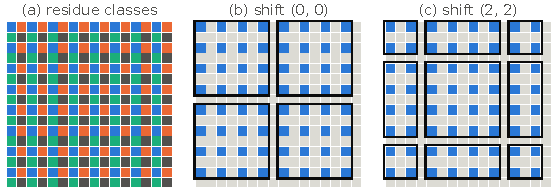
\includegraphics[width=\linewidth]{figures/fig_ref_windows}\par\smallskip
{\small At stride $(s_x,s_y)$ the cells fall into $s_xs_y$ residue classes $(x \bmod s_x,\,
y \bmod s_y)$ (a). In its class, cell $x$ is lattice column $x /\!/ s_x$, and tiles of $w$
lattice columns start at column \texttt{ox}. A window is the set of cells that share a class
and a tile (b, boxes). The four tilings of a round shift the tiles by half a window (c). Edge
windows are smaller, and masked cells never appear. Drawn with $w=4$, stride 2, class
$(0,0)$.\par}
\end{minipage}\hfill
\begin{minipage}[t]{0.565\linewidth}\vspace{0pt}
\lstinputlisting[firstline=37,lastline=44,firstnumber=37,numbers=left,numberstyle=\tiny\color{black!45},numbersep=6pt,frame=none,xleftmargin=1.6em,aboveskip=0pt,belowskip=0pt]{reference.py}
\end{minipage}

\vspace{1.4em}
\noindent\begin{minipage}[t]{0.405\linewidth}\vspace{0pt}\raggedright
\textbf{One window.}\par\smallskip
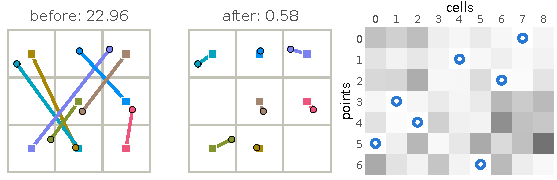
\includegraphics[width=\linewidth]{figures/fig_ref_solve}\par\smallskip
{\small The window's points are reassigned among all of its cells, empty ones included, by an
exact linear assignment on squared distances. The result is kept only if it lowers the
window's cost by more than a relative \texttt{tol}, so the cost never rises and ties cannot
cycle. \texttt{pos} gives each point's cell and \texttt{occ} each cell's point. Drawn: seven
points in a $3\times3$ window before and after, with summed squared distances, and the cost
matrix with the chosen entries.\par}
\end{minipage}\hfill
\begin{minipage}[t]{0.565\linewidth}\vspace{0pt}
\lstinputlisting[firstline=47,lastline=59,firstnumber=47,numbers=left,numberstyle=\tiny\color{black!45},numbersep=6pt,frame=none,xleftmargin=1.6em,aboveskip=0pt,belowskip=0pt]{reference.py}
\end{minipage}

\clearpage
\noindent\begin{minipage}[t]{0.405\linewidth}\vspace{0pt}\raggedright
\textbf{The whole method.}\par\smallskip
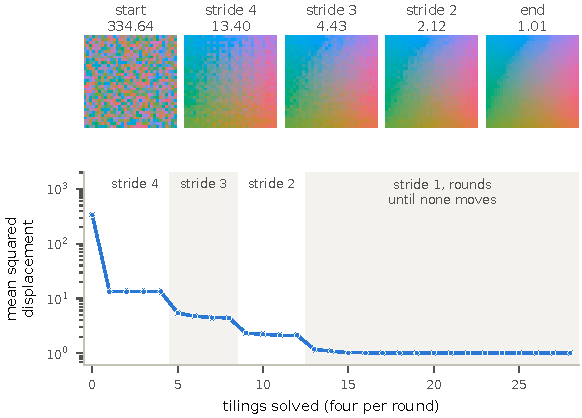
\includegraphics[width=\linewidth]{figures/fig_ref_snap}\par\smallskip
{\small The cells are the mask's usable entries in row-major order, and point $i$ starts in a
random cell \texttt{pos[i]}. A round solves the windows of the four tilings in turn. Each
coarse stage runs one round; then stride-1 rounds repeat until one moves nothing, a fixed
point of every window but not a proof of optimality. Drawn: 1{,}024 uniform points on a
$32\times32$ grid, colored by input position, after the start, each
coarse stage and the end (top), and the mean squared displacement in cells$^2$ after every
tiling (bottom): each stride halves it or better, and the last stride-1 round moves
nothing.\par}
\end{minipage}\hfill
\begin{minipage}[t]{0.565\linewidth}\vspace{0pt}
\lstinputlisting[firstline=62,lastline=83,firstnumber=62,numbers=left,numberstyle=\tiny\color{black!45},numbersep=6pt,frame=none,xleftmargin=1.6em,aboveskip=0pt,belowskip=0pt]{reference.py}
\end{minipage}
\end{landscape}


\section{Additional tables}
\label{app:tables}

\begin{table}[tbp]
\centering\scriptsize
\setlength{\tabcolsep}{3.2pt}
\caption{Absolute excess over the certified optimum, in cells$^2$ per point, at $N=100{,}000$
(same runs as Table~\ref{tab:main}). ``Optimum'' is the certified optimal mean squared
displacement. Relative and absolute excess tell different stories on the heavy-tailed
input, where outliers dominate the optimum.}
\label{tab:abs}
\resizebox{\linewidth}{!}{\begin{tabular}{lrrrrrrrrr}
\toprule
distribution & optimum & SS fast & BSP 16 & SS bal. & BSP 64 & SS qual. & RF master & RF PyPI & Bisect. \\
\midrule
uniform & 1.80 & 0.045 & 0.80 & 0.015 & 0.58 & 0.008 & 0.80 & 1.10 & 1.81 \\
Gaussian & 6501 & 0.030 & 3.61 & 0.011 & 2.60 & 0.005 & 0.38 & 0.66 & 1.17 \\
Gaussian mixture & 4440 & 0.58 & 252 & 0.11 & 167 & 0.010 & 751 & 752 & 554 \\
90/10 clusters & 8743 & 4.34 & 2.77 & 1.01 & 1.66 & 0.079 & 102 & 101 & 49.9 \\
ring & 1731 & 0.081 & 20.1 & 0.022 & 16.5 & 0.008 & 710 & 710 & 697 \\
spiral & 1338 & 0.29 & 133 & 0.055 & 108 & 0.015 & 366 & 367 & 460 \\
checkerboard & 32.1 & 0.041 & 16.0 & 0.018 & 11.6 & 0.006 & 137 & 137 & 145 \\
heavy tails & 32818 & 0.009 & 0.019 & 0.007 & 0.012 & 0.005 & 0.018 & 0.070 & 0.059 \\
duplicates & 4136 & 5.88 & 491 & 1.45 & 228 & 0.47 & 2034 & 2035 & 1645 \\
near-line & 9876 & 0.98 & 0.81 & 0.21 & 0.20 & 0.033 & 1912 & 1912 & 1884 \\
\bottomrule
\end{tabular}
}
\end{table}

\begin{table}[tbp]
\centering\scriptsize
\setlength{\tabcolsep}{3.2pt}
\caption{As Table~\ref{tab:main}, at $N=10{,}000$. Here the dense SciPy solver is feasible; the
last column gives its time on instance seed 1 (it returns the same optimum as the
certified solver).}
\label{tab:main10k}
\resizebox{\linewidth}{!}{\begin{tabular}{lrrrrrrrrrr}
\toprule
distribution & SS fast & BSP 16 & SS bal. & BSP 64 & SS qual. & RF master & RF PyPI & Bisect. & exact (s) & dense (s) \\
\midrule
uniform & 2.34 & 27.6 & 0.69 & 17.9 & 0.28 & 31.8 & 82.4 & 86.2 & 0.53 & 10.8 \\
Gaussian & 0.003 & 0.13 & 0.001 & 0.093 & $<$0.001 & 0.040 & 0.14 & 0.15 & 1.31 & 205 \\
Gaussian mixture & 0.014 & 3.78 & 0.004 & 2.54 & $<$0.001 & 38.7 & 39.7 & 13.1 & 2.05 & 176 \\
90/10 clusters & 0.037 & 0.13 & 0.011 & 0.049 & 0.001 & 1.32 & 1.47 & 0.66 & 2.91 & 227 \\
ring & 0.018 & 3.78 & 0.007 & 1.56 & 0.005 & 40.5 & 41.6 & 39.4 & 1.92 & 104 \\
spiral & 0.036 & 10.3 & 0.013 & 7.30 & 0.005 & 24.6 & 29.9 & 31.9 & 2.29 & 84.9 \\
checkerboard & 0.72 & 55.4 & 0.28 & 44.8 & 0.090 & 271.4 & 260.7 & 265.2 & 0.53 & 15.9 \\
heavy tails & $<$0.001 & 0.005 & $<$0.001 & 0.003 & $<$0.001 & $<$0.001 & 0.002 & 0.003 & 3.21 & 352 \\
duplicates & 0.15 & 12.0 & 0.045 & 4.97 & 0.014 & 57.6 & 58.0 & 36.6 & 0.97 & 126 \\
near-line & 0.012 & 0.027 & 0.003 & 0.007 & $<$0.001 & 19.4 & 19.8 & 19.5 & 6.92 & 246 \\
\midrule
\emph{median time (s)} & 0.057 & 0.063 & 0.15 & 0.25 & 0.42 & 0.22 & 0.029 & 0.003 & 1.99 & 151 \\
\bottomrule
\end{tabular}
}
\end{table}

\begin{table}[tbp]
\centering\scriptsize
\setlength{\tabcolsep}{3.2pt}
\caption{As Table~\ref{tab:main}, at $N=50{,}000$.}
\label{tab:main50k}
\resizebox{\linewidth}{!}{\begin{tabular}{lrrrrrrrrrr}
\toprule
distribution & SS base & SS fast & SS bal. & SS qual. & BSP 16 & BSP 64 & RF master & RF PyPI & Bisect. & exact (s) \\
\midrule
uniform & 3.61 & 2.24 & 1.20 & 0.48 & 45.5 & 36.8 & 40.4 & 65.4 & 114.2 & 6.82 \\
Gaussian & $<$0.001 & $<$0.001 & $<$0.001 & $<$0.001 & 0.056 & 0.039 & 0.009 & 0.018 & 0.031 & 38.4 \\
Gaussian mixture & 0.012 & 0.008 & 0.001 & $<$0.001 & 5.47 & 3.83 & 38.2 & 38.2 & 14.6 & 47.6 \\
90/10 clusters & 0.031 & 0.026 & 0.005 & $<$0.001 & 0.049 & 0.025 & 1.21 & 1.22 & 0.86 & 65.1 \\
ring & 0.017 & 0.004 & 0.002 & $<$0.001 & 2.15 & 0.59 & 41.1 & 41.1 & 42.2 & 37.6 \\
spiral & 0.025 & 0.014 & 0.006 & 0.002 & 11.4 & 7.74 & 27.3 & 27.4 & 25.0 & 43.1 \\
checkerboard & 0.29 & 0.16 & 0.085 & 0.035 & 81.6 & 69.4 & 398.0 & 400.1 & 423.4 & 14.4 \\
heavy tails & $<$0.001 & $<$0.001 & $<$0.001 & $<$0.001 & $<$0.001 & $<$0.001 & $<$0.001 & $<$0.001 & $<$0.001 & 92.1 \\
duplicates & 0.11 & 0.083 & 0.038 & 0.013 & 13.8 & 4.91 & 58.6 & 58.6 & 39.7 & 151 \\
near-line & 0.007 & 0.002 & $<$0.001 & $<$0.001 & 0.028 & 0.003 & 19.7 & 19.7 & 19.5 & 77.9 \\
jittered lattice & 24.5 & 17.3 & 13.1 & 6.91 & 59.4 & 41.2 & 12.1 & 27.7 & 205.6 & 2.87 \\
\midrule
\emph{median time (s)} & 2.26 & 3.04 & 6.95 & 22.6 & 0.34 & 1.36 & 1.45 & 12.4 & 0.016 & 43.1 \\
\bottomrule
\end{tabular}
}
\end{table}

\begin{table}[tbp]
\centering\scriptsize
\setlength{\tabcolsep}{3.2pt}
\caption{RasterFairy's swap optimizer (upstream \texttt{rfoptimizer.py}) at $N=2{,}500$
($50\times50$ grid), mean excess over the certified optimum (\%) over instance seeds 1--3,
one thread. RF is RasterFairy upstream; the next four columns run the swap optimizer from its
layout for $10^4$ to $10^7$ iterations, and the last one from a random permutation, as in
upstream's demo. \textsuperscript{a}: timed on another physical core (seed 1) or on five
others in parallel (seeds 2--3). The dense SciPy solver returns the optimum in a median of
2.7\,s.}
\label{tab:swap}
\resizebox{\linewidth}{!}{\begin{tabular}{lrrrrrrrrrrr}
\toprule
 & & & & & & & \multicolumn{4}{c}{RF + swap optimizer} & \\
\cmidrule(lr){8-11}
distribution & SS fast & SS bal. & SS qual. & BSP 16 & BSP 64 & RF & $10^4$ & $10^5$ & $10^6$ & $10^7$\textsuperscript{a} & rand.\ $10^6$ \\
\midrule
uniform & 1.56 & 1.05 & 0.30 & 26.8 & 19.3 & 16.6 & 16.6 & 16.2 & 15.2 & 13.9 & 6320 \\
Gaussian & 0.012 & 0.006 & 0.001 & 0.22 & 0.15 & 0.11 & 0.11 & 0.11 & 0.11 & 0.100 & 29.5 \\
Gaussian mixture & 0.033 & 0.012 & 0.002 & 6.06 & 3.58 & 38.3 & 33.7 & 28.7 & 18.1 & 10.4 & 39.3 \\
90/10 clusters & 0.048 & 0.013 & 0.005 & 0.29 & 0.16 & 1.20 & 1.16 & 1.06 & 0.82 & 0.50 & 17.1 \\
ring & 0.053 & 0.018 & 0.004 & 2.95 & 2.24 & 35.9 & 35.3 & 33.2 & 21.5 & 12.3 & 101.7 \\
spiral & 0.13 & 0.036 & 0.012 & 9.64 & 5.53 & 10.4 & 10.3 & 9.97 & 8.82 & 7.16 & 140.0 \\
checkerboard & 1.15 & 0.43 & 0.33 & 51.2 & 36.1 & 56.3 & 56.0 & 52.5 & 45.1 & 33.6 & 4346 \\
heavy tails & $<$0.001 & $<$0.001 & $<$0.001 & 0.006 & 0.004 & 0.003 & 0.003 & 0.003 & 0.002 & 0.002 & 0.43 \\
duplicates & 0.17 & 0.050 & 0.015 & 9.03 & 6.77 & 55.6 & 54.0 & 48.7 & 36.7 & 30.2 & 50.1 \\
near-line & 0.015 & 0.004 & 0.002 & 0.070 & 0.020 & 19.2 & 14.3 & 11.6 & 1.65 & 0.81 & 6.98 \\
\midrule
\emph{median time (s)} & 0.012 & 0.029 & 0.071 & 0.015 & 0.059 & 0.051 & 0.75 & 6.44 & 63.3 & 613 & 61.7 \\
\bottomrule
\end{tabular}
}
\end{table}

\begin{figure}[tbp]
  \centering
  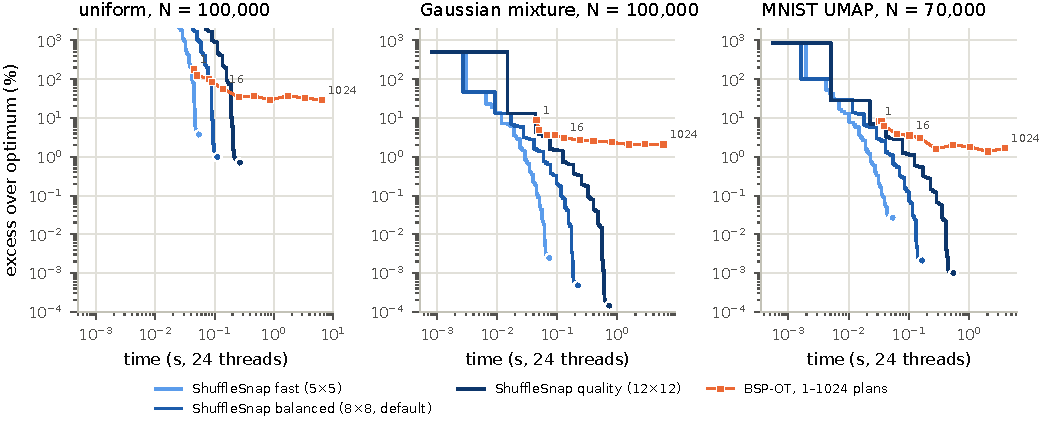
\includegraphics[width=\linewidth]{figures/fig_anytime_t24.pdf}
  \caption{As Figure~\ref{fig:anytime}, with 24 threads for \ShuffleSnap\ and BSP-OT
  (RasterFairy is single-threaded).}
  \label{fig:anytime24}
\end{figure}

\begin{table}[tbp]
\centering\scriptsize
\caption{All held-out ablations (24 threads): mean excess over the certified optimum (\%) and
median time (s) over instance seeds 1--3. Each row changes one setting of the default
($8\times8$ windows, stride ratio $\sqrt2$, four tilings, random start, one round per level,
geometric window solver, unchanged windows skipped, automatic start stride).}
\label{tab:ablation}
\resizebox{\linewidth}{!}{\begin{tabular}{llrrrrrr}
\toprule
change & setting & \multicolumn{2}{c}{uniform 100k} & \multicolumn{2}{c}{mixture 100k} & \multicolumn{2}{c}{MNIST 70k} \\
 & & excess \% & time (s) & excess \% & time (s) & excess \% & time (s) \\
\midrule
window side (ratio 2) & 3$\times$3 & 15.7 & 0.054 & 0.16 & 0.074 & 0.21 & 0.051 \\
 & 4$\times$4 & 6.36 & 0.072 & 0.035 & 0.12 & 0.079 & 0.084 \\
 & 5$\times$5 & 3.71 & 0.098 & 0.022 & 0.22 & 0.031 & 0.14 \\
 & 6$\times$6 & 2.51 & 0.13 & 0.011 & 0.37 & 0.015 & 0.24 \\
 & 7$\times$7 & 1.94 & 0.19 & 0.006 & 0.58 & 0.013 & 0.39 \\
 & 8$\times$8 & 1.52 & 0.25 & 0.004 & 0.87 & 0.004 & 0.59 \\
 & 10$\times$10 & 0.93 & 0.44 & 0.001 & 1.80 & 0.002 & 1.19 \\
 & 12$\times$12 & 0.54 & 0.68 & $<$0.001 & 3.16 & 0.001 & 2.12 \\
 & 16$\times$16 & 0.29 & 1.47 & $<$0.001 & 8.43 & $<$0.001 & 5.72 \\
\addlinespace
window side (ratio $\sqrt2$) & 4$\times$4 & 3.76 & 0.072 & 0.027 & 0.17 & 0.068 & 0.11 \\
 & 6$\times$6 & 1.50 & 0.14 & 0.008 & 0.53 & 0.010 & 0.35 \\
 & 8$\times$8 & 0.84 & 0.25 & 0.002 & 1.25 & 0.002 & 0.81 \\
 & 10$\times$10 & 0.54 & 0.42 & $<$0.001 & 2.49 & 0.002 & 1.55 \\
 & 12$\times$12 & 0.44 & 0.62 & $<$0.001 & 4.33 & $<$0.001 & 2.88 \\
 & 16$\times$16 & 0.19 & 1.32 & $<$0.001 & 11.1 & $<$0.001 & 7.78 \\
\addlinespace
stride ratio & 3 & 4.14 & 0.11 & 0.014 & 0.32 & 0.041 & 0.23 \\
 & 2 (baseline) & 2.51 & 0.13 & 0.011 & 0.37 & 0.015 & 0.25 \\
 & 1.68 & 1.99 & 0.13 & 0.007 & 0.43 & 0.011 & 0.28 \\
 & 1.41 & 1.50 & 0.14 & 0.008 & 0.53 & 0.010 & 0.35 \\
 & 1.19 & 1.58 & 0.17 & 0.009 & 0.80 & 0.013 & 0.50 \\
 & 1.1 & 1.93 & 0.20 & 0.009 & 1.04 & 0.018 & 0.64 \\
\addlinespace
start & random (baseline) & 2.51 & 0.14 & 0.011 & 0.37 & 0.015 & 0.24 \\
 & bisection & 29.9 & 0.16 & 0.21 & 0.73 & 0.14 & 0.33 \\
 & row sort & 22.9 & 0.13 & 0.042 & 1.02 & 0.12 & 0.41 \\
\addlinespace
rounds per level & 1 & 2.51 & 0.14 & 0.011 & 0.37 & 0.015 & 0.24 \\
 & 2 & 2.08 & 0.20 & 0.009 & 0.55 & 0.012 & 0.36 \\
 & 3 & 1.87 & 0.22 & 0.009 & 0.62 & 0.011 & 0.41 \\
\addlinespace
tilings per round & 1 & 21166 & 0.046 & 4.50 & 0.079 & 12.3 & 0.051 \\
 & 2 (diagonal) & 5.49 & 0.076 & 0.029 & 0.20 & 0.031 & 0.14 \\
 & 4 (baseline) & 2.51 & 0.13 & 0.011 & 0.36 & 0.015 & 0.24 \\
 & 9 & 1.86 & 0.27 & 0.006 & 0.76 & 0.008 & 0.51 \\
\addlinespace
first stride & automatic (baseline) & 2.51 & 0.12 & 0.011 & 0.35 & 0.015 & 0.24 \\
 & capped at 16 & 11.7 & 0.57 & 0.29 & 27.2 & 0.44 & 8.88 \\
 & capped at 8 & 10.9 & 0.95 & 0.27 & 29.1 & 0.54 & 11.5 \\
 & capped at 4 & 12.9 & 1.21 & 0.28 & 29.8 & 0.62 & 12.0 \\
 & capped at 2 & 15.7 & 1.30 & 0.28 & 29.6 & 0.58 & 11.1 \\
 & capped at 1 & 27.4 & 1.27 & 0.28 & 31.2 & 0.55 & 11.8 \\
\addlinespace
window solver & Hungarian, 6$\times$6 & 2.51 & 0.15 & 0.011 & 0.36 & 0.015 & 0.24 \\
 & Hungarian + greedy start, 6$\times$6 & 2.51 & 0.14 & 0.011 & 0.37 & 0.015 & 0.24 \\
 & Jonker--Volgenant, 6$\times$6 & 2.51 & 0.29 & 0.011 & 1.53 & 0.015 & 0.88 \\
 & Hungarian, 12$\times$12 & 0.54 & 0.80 & $<$0.001 & 3.13 & 0.001 & 2.14 \\
 & Hungarian + greedy start, 12$\times$12 & 0.54 & 0.68 & $<$0.001 & 3.21 & 0.001 & 2.21 \\
 & Jonker--Volgenant, 12$\times$12 & 0.54 & 5.27 & $<$0.001 & 32.6 & 0.001 & 20.7 \\
\addlinespace
skip unchanged windows & yes (baseline) & 2.51 & 0.14 & 0.011 & 0.36 & 0.015 & 0.24 \\
 & no & 2.51 & 0.21 & 0.011 & 0.59 & 0.015 & 0.41 \\
\bottomrule
\end{tabular}
}
\end{table}


\end{document}
